% Paper 1: structure of best-known Heilbronn configurations in the unit square.
% Every numerical claim carries a hidden "% SRC:" comment naming the lab file it comes from.
% Items to verify are marked "% CHECK"; open items "% PENDING".
\documentclass[11pt]{amsart}

\usepackage[T1]{fontenc}
\usepackage[utf8]{inputenc}
\usepackage{lmodern}
\usepackage{microtype}
\usepackage[margin=2.6cm]{geometry}
\usepackage{amsmath,amssymb,amsthm}
\usepackage{booktabs}
\usepackage{longtable}
\usepackage{array}
\usepackage{xcolor}
\usepackage{graphicx}
\graphicspath{{figures/}}
\usepackage{enumitem}
\usepackage{url}
\usepackage[colorlinks=true,linkcolor=blue!50!black,urlcolor=blue!50!black,citecolor=blue!50!black]{hyperref}

\setlist{itemsep=1pt,topsep=3pt}

\newtheorem{theorem}{Theorem}[section]
\newtheorem{proposition}[theorem]{Proposition}
\newtheorem{lemma}[theorem]{Lemma}
\newtheorem{corollary}[theorem]{Corollary}
\theoremstyle{definition}
\newtheorem{definition}[theorem]{Definition}
\newtheorem{remark}[theorem]{Remark}
\newtheorem{observation}[theorem]{Observation}

\newcommand{\Q}{\mathbb{Q}}
\newcommand{\R}{\mathbb{R}}
\newcommand{\sq}{[0,1]^2}
\newcommand{\core}{\mathrm{core}}
\newcommand{\tr}{\operatorname{tr}}

\begin{document}

\title[Structure of best-known Heilbronn configurations]{The structure of best-known Heilbronn configurations in the unit square: certificates, geometric families and a crossover at $n=43$}

\author{Ethan Hendren}
\email{eehendren007@gmail.com}

\begin{abstract}
For Heilbronn's problem in the unit square (place $n$ points so that the smallest triangle is as large as possible) we study the structure of best-known configurations for $20 \le n \le 100$.
We give configurations for $37 \le n \le 100$, sizes for which we found no published configurations. At every size except $n = 97$ a computer-assisted certificate shows that an exact local maximum, strict in the coordinates of its non-rattler points, lies within about $10^{-30}$ of a polished copy of the stored coordinates (the polished copy differs from them by at most $10^{-11}$ at first-order sizes and by at most $6\cdot10^{-6}$, along the flat direction, at second-order sizes). In these proofs floating point only selects active sets, symmetry and preconditioners; the inequalities they rest on are checked in exact rational or interval arithmetic, except that at $n = 40$ the lift from symmetry-reduced to full variables is a hand argument checked numerically. A separately written check confirms 31 of them (its second-order step is in floating point). Neither code is formally verified.
None of them is claimed to be optimal, and no published record at $n \le 36$ is improved.
On the structural side we prove three short results: a wall-contact theorem (a local maximum that is strict in the coordinates of its non-rattler points has strictly interleaving contacts on each pair of opposite walls), a wall-force law for convex polygons that extends Trela's affine wall identity (in a triangle every side carries the same force, centred at its midpoint), and a group-arithmetic lemma on centre points of symmetric configurations.
Empirically, the best configurations form families that each hold the best value over a window of sizes; up to $n = 42$ every best configuration we know has an empty centre, and from $n = 44$ a search restricted to empty-centre configurations stays well below the filled-centre ones.
We call this a crossover at $n = 43$: a joint breakpoint in measured observables of the best-known configurations, which survives trend and leave-one-family-out controls, and a change of best-known architecture. We do not claim a transition in the global optima.
We also give rigorous computer re-proofs of the known optima $n = 7, 8$, report a computer-assisted proof that the known $n = 9$ configuration is optimal (presented in a companion paper; AI-assisted and not yet independently checked), and give exact algebraic values of the best-known configurations at eleven small sizes; the value for $n = 20$ has degree~19 with Galois group $S_{19}$.
\end{abstract}

\maketitle

% =====================================================================
\section{Introduction}\label{sec:intro}

Let $Q = \sq$ and, for $P = (p_1,\dots,p_n) \in Q^n$, let
\[
  f(P) = \min_{i<j<k} \lvert\Delta(p_i,p_j,p_k)\rvert, \qquad \Delta(a,b,c) = \tfrac12 \det(b-a,\, c-a),
\]
the smallest area of a triangle with vertices in $P$. Heilbronn's problem asks for $H(n) = \max_{P \in Q^n} f(P)$ and for the maximising configurations. Throughout, $t$ denotes the minimum area $f(P)$ of the configuration under discussion; in the tables it is the best value we know at size $n$, and $n^2t$ is its normalised form.

\subsection*{Asymptotics}
Koml\'os, Pintz and Szemer\'edi proved the lower bound $H(n) \ge c \log n / n^2$ \cite{KPS82} and the upper bound $H(n) \le n^{-8/7+\varepsilon}$ \cite{KPS81}.
Cohen, Pohoata and Zakharov improved the upper bound to $n^{-8/7-1/2000}$ \cite{CPZ23}, and then to $n^{-7/6+o(1)}$ \cite{CPZ24}. % SRC: experiments/LITERATURE.md (arXiv sweep); experiments/101-red-team/NOTES.md issue 5
Nothing in the present paper bears on the asymptotics; the range $n \le 100$ is far from it.

\subsection*{Small \texorpdfstring{$n$}{n}}
Optimality was proved for $n \le 8$ by classical methods: $n = 5$ by Yang, Zhang and Zeng \cite{YZZ}, $n = 6$ by Dress, Yang and Zeng \cite{DYZ}, $n = 7$ by Zeng and Chen \cite{ZC}, $n = 8$ by Dehbi and Zeng \cite{DZ}; these are the sources listed by the record site \cite{Stead}. % SRC: experiments/102-laws-small-n (via report_tex/heilbronn_report.tex Sec. 2) % bibliographic data verified 2026-11-12 (record site DOIs, Trela/MMK bibliographies); papers not read
Sudermann-Merx \cite{SM} solves $n \le 10$ by mixed-integer nonlinear programming to global optimality within solver tolerance and gives exact values for $n = 5$--$10$. % SRC: experiments/LITERATURE.md Sec. 1
Monji, Modir and Kocuk \cite{MMK} give MIQCP formulations with symmetry breaking and solve $n \le 9$. % SRC: experiments/LITERATURE.md Sec. 1
For $n = 9$, Chen, Xu and Zeng \cite{Chen17} confined all optimal configurations by a GPGPU search and obtained $0.054875999 < H(9) < 0.054878314$ (as quoted in \cite{MMK}). % SRC: arXiv 2512.14505v1 Introduction; J. Global Optim. 68 (2017) abstract
We give a computer-assisted proof that $H(9) = (9\sqrt{65}-55)/320$, attained uniquely up to the symmetries of the square, by an exact computer-assisted branch and bound in which every discard is decided in exact arithmetic (Section~\ref{sec:smalln}; details in the companion paper \cite{N9}). This proof is AI-assisted and has not yet been independently checked. % SRC: experiments/110-n9-proof/NOTES.md (Result); STATUS.md row 110
Earlier constructions for small $n$ are due to Goldberg \cite{Goldberg} and Comellas and Yebra \cite{CY}.

\subsection*{The record site}
Best-known configurations for $n \le 36$ are collected, with exact rational verification, on the record site maintained by Tej Stead \cite{Stead}. % SRC: report_tex/heilbronn_report.tex Sec. 2
Current record holders listed there are Comellas and Yebra ($n = 7$--$10$, $12$), Goldberg ($11$), Karpov ($13$), Beyleveld ($14$, $16$), Nemri with AlphaEvolve ($17$), ``Fable 5.1 with Shengtong Zhang'' ($18$, $20$), Stead ($19$, $31$), Gardiner ($21$, $23$), Coupvent des Graviers ($32$), Chappell ($35$, and the exact realization of $14$) and Sudermann-Merx ($15$, $22$, $24$--$30$, $33$, $34$, $36$, mostly October 2026). % SRC: math.tejstead.com/heilbronn/square/ read 2026-11-12
At the time of writing the site lists no square configuration for $n \ge 37$. % SRC: math.tejstead.com/heilbronn/square/ (pages n = 3--36 only), re-checked 2026-11-12

\subsection*{Related work}
Trela \cite[Thm.~2.3]{Trela} proves that every local maximum with positive area admits normalized Karush--Kuhn--Tucker (KKT) multipliers and derives an affine wall identity: at a KKT point every side of the square carries total wall force equal to the minimum area \cite[eq.~(17)]{Trela}, and opposite sides have equal first moments of wall force \cite[eq.~(18)]{Trela}, hence equal force centroids. % SRC: experiments/LITERATURE.md Sec. 1; 99-wall-contact-bound/NOTES.md Sec. 5
We re-derived this identity independently before finding it there; it is Trela's, and we use it throughout.
The counting of active constraints at an optimum is the Heilbronn case of the classical minimax and isostatic counting; cf.\ Connelly, Gortler, Solomonides and Yampolskaya \cite{CGSY} for jammed disk packings, and Donev, Torquato, Stillinger and Connelly \cite{DTSC}. % SRC: experiments/LITERATURE.md (exp 94 addendum)
Sudermann-Merx derives from that count his conjecture that at least one optimal configuration has at least $2n-7$ minimal triangles \cite[Conj.~1]{SM} (the conjecture is existential; N.~Sudermann-Merx, personal communication, 13 November 2026); the companion note \cite{Note2} discusses it.
Families of optimal patterns that hold over a range of sizes and are then replaced are well known for dense packings of equal disks in a square (Graham and Lubachevsky \cite{GL}) and for Lennard-Jones clusters (Wales and Doye \cite{WD}, Doye, Miller and Wales \cite{DMW}); the appearance of a central particle in two-dimensional confined Coulomb clusters (Bedanov and Peeters \cite{BP}) is the closest physical analogue of the crossover we describe in Section~\ref{sec:43}. % SRC: experiments/LITERATURE.md Sec. 3 and exp 94 addendum
Heilbronn's problem also serves as a benchmark for AI-assisted search (AlphaEvolve \cite{AlphaEvolve}, FlowBoost \cite{FlowBoost}, GigaEvo \cite{GigaEvo}); we mention these only as benchmarks. As far as we could see, none of them discusses empty centres, crossovers, families or critical-triangle counts. % SRC: experiments/LITERATURE.md (read 2026-11-12)
We found no structural study of Heilbronn configurations beyond $n = 16$. % SRC: report_tex Sec. Phase 4 item 4 (exp 94 novelty check)

\subsection*{Contributions}
We separate what is ours from what is re-derived or known.
\begin{enumerate}[label=(\arabic*)]
\item \emph{Configurations for $37 \le n \le 100$} (ours), with exact values and local-maximality certificates at every size except $n = 97$ (Section~\ref{sec:results}). They are first entries, not improved records, and from about $n = 45$ on they are probably far from optimal. One of them ($n = 40$) has been submitted to the record site and is under review. % SRC: MEMORY (PR #78), report_tex Sec. Status at a glance
\item \emph{Certification} (method adapted from standard Krawczyk / radii-polynomial existence tests; implementation ours): two independently written codes; Section~\ref{sec:cert} states which steps are exact and which are not.
\item \emph{Three short theorems} (Section~\ref{sec:theory}): the strict interleaving of wall contacts (ours; the weaker intersection condition is Sudermann-Merx's \cite[Lemma~2(C)]{SM}); the wall-force law for triangles and convex polygons (ours, a direct consequence of Trela's identity); the group-arithmetic lemma (elementary; we state it because it is used). The counting bound of Proposition~\ref{prop:dof} is rank--nullity and is classical; what we add is the empirical observation that it is tight at 36 of 44 sizes and that the number of flat directions is at most one.
\item \emph{Empirical structure} (ours): families and their windows; an empty-centre phase up to $n = 42$ and a crossover at $n = 43$ (a breakpoint in the measured best-known configurations and a change of best-known architecture, with its controls; not a claim about global optima); the absence of a robust second breakpoint up to $n = 100$ (Sections~\ref{sec:families}--\ref{sec:43}).
\item \emph{Small $n$} (Section~\ref{sec:smalln}): rigorous computer re-proofs of the known optima $n = 7, 8$ (known results; independent method), a summary of our computer-assisted proof for $n = 9$ \cite{N9} (AI-assisted, not yet independently checked), and exact values of the best-known configurations at eleven small sizes. Of these, $n = 5$--$11$ and $16$ are known, $n = 12$ is in Comellas--Yebra \cite{CY}, $n = 14$ is on the record site (Chappell \cite{Chappell}); the degree-19 value at $n = 20$ was not found in the literature we read (the record site's $n = 20$ history gives a degree-20 polynomial as the exact value, but the record value is not a root of it, and its root is the value of a different, lower $n = 20$ configuration; see Section~\ref{sec:smalln}).
\item \emph{Other regions} (Section~\ref{sec:regions}): the laws in triangles, the record site's convex-hull variant, regular hexagons and pentagons and the disk; a test that refutes our own earlier half-turn explanation of the empty centre.
\end{enumerate}

% =====================================================================
\section{Definitions and methods}\label{sec:methods}

\subsection{KKT points, core and rattlers}
Near a configuration $P$ with $f(P) = t > 0$ the orientation $\sigma_T \in \{\pm1\}$ of every triangle $T$ is fixed, so locally $f$ is the value of
\begin{equation}\label{eq:nlp}
  \max\ \tau \quad\text{s.t.}\quad \sigma_T \Delta_T(P) \ge \tau \ \ (\text{all } T), \qquad 0 \le x_i, y_i \le 1 .
\end{equation}
A \emph{KKT pair} at $P$ consists of $\lambda_T \ge 0$ on tied triangles (those with $\sigma_T\Delta_T = t$), $\sum_T \lambda_T = 1$, and $\mu_c \ge 0$ on wall contacts $c$ (a point lying on a side), with $\sum_T \lambda_T \nabla(\sigma_T\Delta_T) + \sum_c \mu_c\, a_c = 0$, where $a_c$ is the inward unit normal of the wall of $c$. By \cite{Trela} every local maximum of $f$ with $f > 0$ admits a KKT pair. % SRC: experiments/LITERATURE.md Sec. 1 (Trela: KKT existence via MFCQ)

\begin{definition}
Fix the KKT pair in the relative interior of the set of KKT pairs (a polytope; all of its relative-interior points have the same set of positive multipliers, so the following notions are well defined). A tie or wall contact is \emph{loaded} if its multiplier is positive. The \emph{core} is the set of points that belong to a loaded constraint; the other points are \emph{rattlers}. We write $\core$ also for the number of core points. Let $J$ be the Jacobian of the loaded constraints with respect to $(\text{core coordinates}, \tau)$, and $d = \dim\ker J$, the number of first-order \emph{flat directions}.
\end{definition}

At symmetric sizes where the multipliers are not unique, our certificates work with a vertex of the multiplier polytope, whose loaded set can be smaller than that of the relative interior; core and rattler counts reported at those sizes ($24, 26, 28, 30, 32, 36, 38, 42$) refer to that vertex.

A rattler lies on no loaded constraint, but it may lie on unloaded ties. At every configuration with rattlers that we certified, except one degenerate $n = 46$ configuration of an earlier library, an LP finds a motion of the rattlers alone that makes all ties through them strictly larger and so leaves $f$ unchanged (experiment~78b); such a configuration is not a strict local maximum, and at best it is strict in the core coordinates. % SRC: experiments/78-independent-certificate/NOTES.md (78b) Of the 44 best configurations for $21 \le n \le 64$, 28 have rattlers; every one of the 40 certified configurations for $60 \le n \le 100$ has rattlers. % SRC: experiments/101-red-team/NOTES.md issue 10 (check_certs.txt)

\begin{definition}
A tie is \emph{critical} in the exact sense if its area equals $t$ exactly at the certified exact optimum. Counts ``within $10^{-6}$'' are relative tolerance counts. They exceed the exact count by near-ties (triangles $2\cdot10^{-9}$--$4\cdot10^{-8}$ above $t$ at the exact optimum), and the exact count exceeds the number of loaded ties by the unloaded ties through rattlers. The companion note \cite{Note2} discusses these conventions in detail. % SRC: experiments/78-independent-certificate/NOTES.md (78b)
\end{definition}

\subsection{Search}\label{sec:search}
Our engine is described only briefly; the structural results do not depend on it. Its core is a sequential linear programming refiner (linearise the near-minimal triangles, solve an LP, repeat), basin hopping, and searches restricted to symmetry classes ($D_4$, $C_4$, $C_2$, mirrors). For growth from $n-1$ to $n$ the decisive moves were collective: \emph{shift-insert} (translate all points by $0.003$--$0.01$, clamped to the square, and insert new points on the walls the shift emptied), a uniform shrink by 1--6\% followed by insertion into the freed band, and a container-free insertion followed by an affine map of the smallest enclosing parallelogram onto the square (adapted from the record holder's convex-variant transfer; it is exact because affine maps preserve area ratios, as used in the proof of \cite[Lemma~1]{SM}). % SRC: report_tex/heilbronn_report.tex Sec. Innovations items 1, 6b
Later gains used a kick that lifts the points to three dimensions with random heights and lets the heights shrink to zero, and a Danzer-type flip (reflect a point in the line through two tied partners). % SRC: report_tex Sec. Phase 3 (exp 80, 83, 84)
Every value reported is recomputed in exact rational arithmetic on the stored coordinates.

As a check of search quality, our searches reproduce the published record values for $19 \le n \le 36$ from independent starts at 12 of the 18 sizes (6 from our own structures, 6 from a neighbouring record); the other 6 were reached only by shrinking and regrowing the record itself, which is a consistency check, not a rebuild. % SRC: report_tex Sec. Status 19-36 table; experiments/101-red-team/NOTES.md issue 14
For $n = 5$--$18$ all record configurations were rebuilt without the site's coordinates (exact minimum within $2\cdot10^{-13}$ relative of the site's, with matching tie and wall-contact counts). % SRC: STATUS.md row 102

\subsection{Exact certification}\label{sec:cert}
The certificate (our experiment~44) proves that an exact local maximum exists near the stored coordinates. % SRC: experiments/44-interval-certificate/NOTES.md
\begin{enumerate}[label=(\roman*)]
\item The symmetry group $G$ of the core is detected; the core is parametrised as $p_j(u) = a_j + B_j u$ with exact rational $a_j, B_j$, keeping loaded wall contacts on their walls and respecting $G$.
\item The reduced tie system $\sigma_k\Delta_{T_k}(p(u)) - \tau = 0$ (one equation per $G$-orbit of loaded ties) is polished by Newton's method on a dyadic grid to residual $\approx 10^{-31}$.
\item Existence and uniqueness of a zero $w^*$ in a sup-ball $B(\tilde w, r)$ follow from the radii-polynomial (Krawczyk-type) inequalities $Y + Z_0 r + Z_2 r^2/2 \le r$ and $Z_0 + Z_2 r < 1$, where $Y = \lVert R F(\tilde w)\rVert_\infty$, $Z_0 = \lVert I - R\,DF(\tilde w)\rVert_\infty$, and $Z_2$ bounds the constant second derivative (the system is quadratic). All bounds are computed exactly; floats only choose $R$, the active set, the symmetry and the stress vertex, so a wrong choice can make the proof fail but cannot make a false proof pass. Radii are $r \approx 10^{-33}$--$10^{-30}$.
\item Every other triangle is proved to exceed $t$ on the ball, and free coordinates are proved to lie strictly inside $(0,1)$. Ties forced by symmetry or by exact polynomial identities (for example the parallelograms of centrally symmetric cores) are identified exactly.
\item \emph{First order} ($d = 0$): a vertex stress with exactly $2\,\core + 1$ rows is shown to have positive multipliers, which gives a proven basin radius ($\sim10^{-10}$--$10^{-6}$ at $n \ge 21$; about $10^{-4}$ at $n = 7, 8$). \emph{Second order} ($d = 1$): the KKT system in $(u,\tau,\lambda)$ is certified by the same Krawczyk test, the multipliers are shown to be positive, and the second-order sufficient condition (the Lagrangian Hessian negative on the flat direction) is proved with an exact lower bound on its margin.
\end{enumerate}
If a triangle through a rattler is not provably above $t$, the rattlers alone are moved (by at most $10^{-4}$, via an LP); the certified configuration is then the exact core plus the moved rattlers, with the same minimum. % SRC: experiments/44-interval-certificate/NOTES.md step 6
Wrong active sets were rejected in 18 of 18 deliberate tests. The certificate concerns the polished point: the stored double-precision configuration differs from it by at most $10^{-11}$ (sup norm, core points) at the first-order sizes, and by $10^{-7}$--$6\cdot10^{-6}$ at the second-order sizes, where the polish moves along the flat direction; the minimum areas agree to $5\cdot10^{-9}$ (relative) or better. % SRC: recomputed in this review from 44-interval-certificate/results/polished/n*.json vs elites and verified.json % SRC: report_tex Sec. Innovations item 7

An \emph{independent} check (experiment~78) uses separately written code: no reduction and no symmetry, the full KKT system in (core coordinates, $\tau$, one multiplier per loaded constraint), a Newton--Kantorovich test in exact rationals around a point refined on a $2^{-180}$ grid (radius $\approx 6\cdot10^{-55}$), and the same post-checks. It agreed with experiment~44 on loaded ties, loaded walls, core and verdict at all 35 sizes in $20$--$64$ where both applied in the library of its first run, and again on the 17 current bests that were re-run on 2026-11-12 and on the current $46, 49, 51, 53, 62$. Of the current bests for $21 \le n \le 64$ it covers 36 of 44; outside its scope are the 8 symmetric sizes with non-unique multipliers. At the second-order sizes $65, 76, 81, 89, 100$ it was run on the polished centres of experiment~44 and agrees there too ($d = 1$, negative eigenvalue). Started from the stored coordinates at these five sizes it does not certify (singular system at 76, 89, 100; a triangle below $t$ at 65, 81): the stored points lie $10^{-7}$--$6\cdot10^{-6}$ from the KKT point along the flat direction, outside its $10^{-9}$ tie window. This is a failure to start, not a contrary verdict. % SRC: 78-independent-certificate/compare.txt, recheck_2026-11-12.txt, results/kkt_certs.jsonl (t matched against elites in this review) % SRC: experiments/78-independent-certificate/NOTES.md
\emph{What is rigorous.} In experiment~44, floating point only selects the active (loaded) sets, the symmetry group, the stress vertex and the preconditioners $R$. Existence and uniqueness of the exact zero (the Krawczyk test), the exact ties, the bound that every other triangle exceeds $t$ on the ball, the positivity of the multipliers and the basin radius are computed in exact rational or interval arithmetic; in second-order mode so are the Krawczyk test of the KKT system, $\lambda > 0$, $\mu > 0$ and the margin in the second-order sufficient condition. One step is not of this kind: at the symmetric second-order sizes $22$ and $24$ (both records) the KKT system is certified in the symmetry-reduced variables, and the lift of the reduced KKT point to a KKT point of the full system is a hand argument (invariance of the full Lagrangian gradient under the symmetry group), checked numerically (residual $\le 2\cdot10^{-33}$). Our $n = 40$ is also certified in reduced variables (group of order 4) and rests on the same argument (full stationarity residual $2\cdot10^{-35}$). % SRC: experiments/44-interval-certificate/NOTES.md (Lifting to full space; line 158); results/certs_report.jsonl n=40 (symmetry id/rot180/diag/antidiag, full_stationarity_residual_centre 2.06e-35); STATUS.md row 108
In experiment~78 every step is exact except the second-order eigenvalues, which are computed in floating point on an exactly computed tangent space (margins $\ge 2.4\cdot10^{-5}$, at $n = 100$) and are not interval-enclosed. % SRC: experiments/78-independent-certificate/NOTES.md (Caveat)
Neither code is formally verified, and neither says anything about global optimality. Appendix~\ref{app:repro} lists, for every $21 \le n \le 100$, which certificate and which independent check apply.

% =====================================================================
\section{Three short theorems}\label{sec:theory}

Throughout, $P \in Q^n$, $n \ge 3$, and $f(P) = t > 0$; in particular the points are distinct and not all collinear. For a wall $w$ let $C_w$ be the set of points of $P$ on $w$ (a corner point lies on two walls). Since three points on a line span zero area, $|C_w| \le 2$.

\subsection{Affine motions}

\begin{lemma}[affine paths]\label{lem:affine}
Let $A \in \R^{2\times2}$, $b \in \R^2$, and $T_\varepsilon(p) = p + \varepsilon(Ap+b)$.
\begin{enumerate}[label=(\alph*)]
\item Every signed area is multiplied by $\det(I+\varepsilon A) = 1 + \varepsilon \tr A + \varepsilon^2 \det A$; hence $f(T_\varepsilon P) = \lvert\det(I+\varepsilon A)\rvert\, f(P)$.
\item Write $v = Ap + b = (\ell(p), m(p))$. Then $T_\varepsilon P \in Q^n$ for all $\varepsilon \in [0,\varepsilon_0]$, for some $\varepsilon_0 > 0$, if and only if $\ell \ge 0$ on $C_L$, $\ell \le 0$ on $C_R$, $m \ge 0$ on $C_B$ and $m \le 0$ on $C_T$. Such $(A,b)$ are called \emph{admissible}.
\item If $(A,b) \ne 0$ then $T_\varepsilon P \ne P$ for every $\varepsilon > 0$.
\end{enumerate}
\end{lemma}

\begin{proof}
(a) $\Delta(T_\varepsilon a, T_\varepsilon b, T_\varepsilon c) = \det(I+\varepsilon A)\Delta(a,b,c)$ because $T_\varepsilon$ is affine with linear part $I+\varepsilon A$.
(b) Each coordinate of $T_\varepsilon p_i$ is affine in $\varepsilon$; coordinates not on a wall have slack, and a coordinate on a wall stays in $[0,1]$ for small $\varepsilon \ge 0$ exactly when its velocity points inward or along the wall.
(c) The points span $\R^2$ affinely (they are not collinear), and an affine map that fixes three non-collinear points is the identity; $T_\varepsilon$ fixes all of $P$ only if $\varepsilon(Ap+b) = 0$ on $P$, i.e.\ $(A,b) = 0$.
\end{proof}

The admissible set is a product $K_x \times K_y$: the first row $\ell(x,y) = ax + cy + e$ is constrained only by $C_L, C_R$, and the second row only by $C_B, C_T$.

\begin{lemma}[one pair of walls]\label{lem:pair}
Let $U, V \subset [0,1]$ be finite (the tangential coordinates of the contacts on the near wall $u=0$ and the far wall $u=1$), and consider $\ell = a u + g(w)$ with $g(w) = cw + e$, admissible if $g \ge 0$ on $U$ and $a + g \le 0$ on $V$.
\begin{enumerate}[label=(\alph*)]
\item An admissible $\ell$ with $a > 0$ exists if and only if $U = \emptyset$, or $V = \emptyset$, or $\max V < \min U$, or $\max U < \min V$.
\item A nonzero admissible $\ell$ with $a \ge 0$ exists if and only if $U = \emptyset$, or $V = \emptyset$, or $\max V \le \min U$, or $\max U \le \min V$.
\end{enumerate}
\end{lemma}

\begin{proof}
(a) If $V = \emptyset$ take $\ell = u$. If $U = \emptyset$ take $a = 1$, $g \equiv -1$. If $\max V < w^* < \min U$, take $g = w - w^*$ and $a = \min_{w\in V}(w^*-w) > 0$; the mirror case is symmetric. Conversely, let $U, V \ne \emptyset$ and $a > 0$. Then $g \ge 0$ on $U$ and $g \le -a < 0$ on $V$, so $g$ is not constant. If $c > 0$, $g$ is increasing with a zero $w^*$, so $U \subset [w^*,\infty)$ and $V \subset (-\infty,w^*)$, whence $\max V < \min U$; $c < 0$ is the mirror case.
(b) If $a > 0$ use (a). If $a = 0$, then $g \ge 0$ on $U$, $g \le 0$ on $V$ and $g \not\equiv 0$. With $U, V$ nonempty a constant $g$ would vanish, so $g$ is strictly monotone with a zero $w^*$ that weakly separates $U$ and $V$. Conversely $g = \pm(w-w^*)$ works.
\end{proof}

\subsection{Strict interleaving of wall contacts}
For the left and right walls let $Y_L, Y_R$ be the heights of the contacts; for the bottom and top walls let $X_B, X_T$ be their abscissae.

\begin{theorem}[wall-contact interleaving]\label{thm:interleave}
Let $P$ be a local maximum of $f$ that is \emph{strict in the coordinates of its core}: some neighbourhood $U$ of $P$ contains no $P' \ne P$ with $f(P') \ge f(P)$ that differs from $P$ in a core point (rattlers may move). Then on each pair of opposite walls the contacts strictly interleave:
\[
  \min Y_L < \max Y_R,\quad \min Y_R < \max Y_L,\qquad \min X_B < \max X_T,\quad \min X_T < \max X_B .
\]
Consequently every wall is touched, $|C_L| + |C_R| \ge 3$ and $|C_B| + |C_T| \ge 3$, so there are between $6$ and $8$ wall incidences (a corner point counted on both of its walls), and if one wall of a pair carries a single contact at height $y$, the opposite wall carries one contact strictly below $y$ and one strictly above.
\end{theorem}

\begin{proof}
Suppose interleaving fails on the pair $L,R$ (the other pair is the same). Then $Y_L$ and $Y_R$ are weakly separated or one is empty, so Lemma~\ref{lem:pair}(b) gives a nonzero admissible $\ell$ with $a \ge 0$. Take $(A,b)$ with first row $\ell$ and second row $0$; then $\tr A = a$ and $\det A = 0$, so by Lemma~\ref{lem:affine}(a) $f(T_\varepsilon P) = (1+\varepsilon a) f(P) \ge f(P)$, and $T_\varepsilon P \in Q^n$ for small $\varepsilon \ge 0$ by Lemma~\ref{lem:affine}(b). A KKT pair exists \cite{Trela} and $\sum_T\lambda_T = 1$, so the core contains the three vertices of a loaded tie, which are not collinear; so a nonzero affine motion moves at least one core point (as in Lemma~\ref{lem:affine}(c)). Hence $T_\varepsilon P$ differs from $P$ in the core coordinates, tends to $P$, and has $f \ge f(P)$: $P$ is not strict in the core coordinates. The counting statements follow because interleaving is impossible with an empty wall or with one contact on each wall.
\end{proof}

\begin{remark}[scope and credit]
(i) The weaker statement that the ranges $[\min Y_L,\max Y_L]$ and $[\min Y_R,\max Y_R]$ intersect is Sudermann-Merx's \cite[Lemma~2(C)]{SM}, stated there for a convex polygon whose minimum-area enclosing parallelogram is the square, which holds for the hull of every optimal configuration by \cite[Lemma~1]{SM}. We did not find the strict version elsewhere (it is not in \cite{Trela} either). % SRC: experiments/99-wall-contact-bound/NOTES.md Sec. 5
(ii) The theorem needs strictness in the core. In our library 145 KKT-clean configurations (top three per $n$ for $20 \le n \le 64$ and the records $19$--$36$) were checked; 144 strictly interleave, and the exception (the second-ranked $n = 32$ configuration) is not strict: the shear $y \mapsto y + c(x - 0.0976)$ keeps it in the square for $c \in [0, 0.0152]$ with all areas unchanged, a segment of equal-value KKT points. % SRC: experiments/99-wall-contact-bound/NOTES.md Sec. 4
Interleaving also holds for every current best $19 \le n \le 100$ and at every certified strict maximum for $5 \le n \le 36$, including the proven optima $n = 5, 7, 8, 9$. % SRC: experiments/101-red-team/NOTES.md (what checks out); STATUS.md row 102
(iii) The count $3$ per pair is attained: 52 library configurations have 6 wall incidences. % SRC: experiments/99-wall-contact-bound/NOTES.md Sec. 3 (Sharpness)
\end{remark}

For loaded contacts the identity of Trela gives a dichotomy.

\begin{proposition}[Trela's wall identity {\cite[eq.~(17)--(18)]{Trela}}]\label{prop:trela}
At a KKT pair of $P$,
\[
  \textstyle\sum_{L}\mu = \sum_{R}\mu = \sum_{B}\mu = \sum_{T}\mu = t, \qquad \sum_L \mu\, y = \sum_R \mu\, y, \qquad \sum_B \mu\, x = \sum_T \mu\, x .
\]
\end{proposition}

\begin{proof}[Proof (re-derivation)]
Contract the stationarity condition with an affine velocity field $v(p) = Ap + b$. Each loaded tie changes at rate $\tr A \cdot t$ by Lemma~\ref{lem:affine}(a), and $\sum\lambda = 1$, so
\begin{equation}\label{eq:virial}
  t \tr A + \textstyle\sum_c \mu_c\, a_c \cdot (A p_c + b) = 0 \qquad \text{for all } A, b .
\end{equation}
Equivalently $\sum_c \mu_c a_c = 0$ and $\sum_c \mu_c\, a_c p_c^{\mathsf T} = -t I$. With $a_L = (1,0)$, $a_R = (-1,0)$, $a_B = (0,1)$, $a_T = (0,-1)$ and $p = (0,y), (1,y), (x,0), (x,1)$ on the four walls, the entries of these two identities are exactly the stated equations.
\end{proof}

\begin{corollary}[loaded contacts]\label{cor:loaded}
At a KKT pair every wall carries a loaded contact. On each pair of opposite walls the loaded contacts either number at least three and strictly interleave, or are exactly one on each wall at the same coordinate $\bar y$. In the latter case the shear $x \mapsto x + s(y-\bar y)$ (or its analogue for the other pair) lies in $\ker J$ and keeps every area constant, so $d \ge 1$ and the Lagrangian Hessian vanishes on it. In particular a configuration with $d = 0$, or with a second-order certificate, has between $6$ and $8$ loaded wall constraints (a corner point can carry one on each of its two walls).
\end{corollary}

\begin{proof}
Each wall has total load $t > 0$. If a pair carries at least three loaded contacts, the positive-weight means of the heights on the two walls coincide; a weighted mean of two distinct heights lies strictly between them, which gives strict interleaving. If it carries one contact on each wall, both means are single heights, so they are equal. A shear fixing the line $y = \bar y$ keeps both contacts on their walls and moves no point across the other two walls, has $\tr A = 0$ and $\det A = 0$, and so preserves every area exactly; restricted to the core it is nonzero (the core has three non-collinear points) and annihilates every loaded constraint, so it lies in $\ker J$. Unloaded contacts may leave the square along it, which does not affect $J$. Areas are constant and the wall constraints linear along the shear, so the Lagrangian Hessian vanishes on it, which excludes a second-order certificate.
\end{proof}

\subsection{A wall-force law for convex polygons}
Let $K$ be a convex polygon with sides $w = 1,\dots,k$, side lines $\{p : a_w\cdot p = \beta_w\}$ with inward unit normals $a_w$, and $K = \{p : a_w \cdot p \ge \beta_w \ \forall w\}$. Problem~\eqref{eq:nlp} in $K$ has the same KKT structure (the Mangasarian--Fromovitz condition holds as in \cite{Trela}: move every point toward an interior point $o$, $p \mapsto p + \varepsilon(o-p)$, and lower $\tau$ at rate $3t$; every active wall constraint then increases at a positive rate, and every tie constraint $\sigma_T\Delta_T - \tau$ at rate $3t - 2t > 0$). Let $F_w = \sum_{c \in w} \mu_c$ be the total force on side $w$ and $s_w$ its force centroid (the $\mu$-weighted mean of the contact points on $w$, defined when $F_w > 0$). % SRC: experiments/105-shape-universality/theory_tri.md; experiments/107-half-turn-test/NOTES.md (wall law)

\begin{theorem}[polygon wall-force law]\label{thm:polygon}
At a KKT pair of a configuration in $K$ with minimum area $t$:
\begin{enumerate}[label=(\alph*)]
\item $\sum_w F_w a_w = 0$ and $\sum_w F_w\, a_w s_w^{\mathsf T} = -tI$;
\item for every point $o$ in the interior of $K$, $\sum_w F_w\, \rho_w(o) = 2t$, where $\rho_w(o)$ is the distance from $o$ to the line of side $w$; in particular, if $K$ has a circle of radius $\rho$ tangent to all its sides (a triangle, a regular polygon), the total wall force is $\sum_w F_w = 2t/\rho$;
\item the identities in (a) are six linear equations in the $2k$ quantities $F_w$ and $F_w\theta_w$, where $\theta_w$ is the position of $s_w$ along side $w$; hence they leave at least $2k-6$ of the force and centroid parameters undetermined;
\item if $K$ is a triangle, the forces and centroids are uniquely determined: in the normalisation where each wall constraint is the barycentric coordinate $\lambda_w(p) \ge 0$, every side carries force $F_w = 2t$ (with unit normals, $F_w = 2t/h_w$, where $h_w$ is the height of $K$ onto side $w$), and every side's force centroid is its midpoint. Since a side contains at most two points, every side carries either exactly one loaded contact, at its midpoint, or two, strictly on opposite sides of it.
\end{enumerate}
\end{theorem}

\begin{proof}
(a) is \eqref{eq:virial} for the walls of $K$, grouped by side: $\sum_{c\in w}\mu_c\, a_w p_c^{\mathsf T} = F_w\, a_w s_w^{\mathsf T}$.
(b) Translate so that $o = 0$; then $\beta_w = -\rho_w(o)$ and, for $p$ on side $w$, $a_w \cdot p = \beta_w$. Taking the trace of the second identity in (a), $\sum_w F_w\, a_w\cdot s_w = \sum_w F_w \beta_w = -2t$. The value does not depend on $o$ because $\sum_w F_w a_w = 0$.
(c) The first identity has two components and the second four.
(d) Map $K$ affinely onto $T_0 = \{x \ge 0,\ y \ge 0,\ x+y \le 1\}$; barycentric coordinates, ratios of areas and the KKT system (with multipliers rescaled by the determinant) are preserved, so it suffices to treat $T_0$ (identity \eqref{eq:virial} holds for any normalisation of the wall gradients), with constraint gradients $a_L = (1,0)$, $a_B = (0,1)$, $a_H = (-1,-1)$ for the sides $x = 0$, $y = 0$, $x + y = 1$. The first identity gives $F_L = F_B = F_H =: F$. A contact on $x = 0$ is $(0,y)$, on $y = 0$ it is $(x,0)$, on the hypotenuse $(x, 1-x)$; with $\bar y_L, \bar x_B, \bar x_H$ the force centroids the second identity reads
\[
  F\begin{pmatrix} -\bar x_H & \bar y_L - (1-\bar x_H) \\ \bar x_B - \bar x_H & -(1-\bar x_H)\end{pmatrix} = -tI .
\]
The diagonal gives $F\bar x_H = t = F(1-\bar x_H)$, so $\bar x_H = 1/2$ and $F = 2t$; the off-diagonal gives $\bar y_L = 1/2$ and $\bar x_B = 1/2$. A positive-weight mean of contact positions equals the midpoint only if the contacts straddle it.
\end{proof}

\begin{remark}
For the square, (a) is Proposition~\ref{prop:trela}: four forces equal to $t$, opposite centroids equal, two centroid heights free ($2k-6 = 2$). In a triangle there is no freedom at all. The theorem is a direct extension of Trela's identity, which we credit; the triangle and $k$-gon statements we did not find in the sources we read. % SRC: experiments/105-shape-universality/theory_tri.md; STATUS.md rows 105, 107
Numerically, all 25 triangle bests of Section~\ref{sec:regions} have $F/t = 2.000$ with centroids at $0.500$ and exactly two loaded contacts per side, and all 63 hexagon, pentagon and disk bests satisfy $\rho\sum_w F_w/(2t) = 1.000$ (residual of the identities in (a) $\le 2\cdot10^{-6}$). % SRC: STATUS.md row 105; experiments/107-half-turn-test/NOTES.md (wall law, data)
Forces on individual sides of the hexagon and pentagon are not equal unless symmetry forces it ($F/t$ between $0$ and $1.32$ in the hexagon, $0.37$ and $1.14$ in the pentagon). % SRC: experiments/107-half-turn-test/NOTES.md
For the disk $\lvert p\rvert \le R$ the same argument gives $\sum\mu = 2t/R$ and $\sum \mu\, u u^{\mathsf T} = (t/R) I$ over the unit contact normals $u$. % SRC: experiments/107-half-turn-test/NOTES.md
\end{remark}

\subsection{Centre points of symmetric configurations}

\begin{lemma}[group arithmetic]\label{lem:group}
Let $G$ be a finite group of isometries fixing a point $c$, and $P$ a $G$-invariant configuration with $f(P) > 0$.
\begin{enumerate}[label=(\alph*)]
\item If $G$ contains the half-turn about $c$, then $c \notin P$ and $n$ is even. If moreover $P \subset Q$ and $c = (\tfrac12,\tfrac12)$ is the centre of the square, the distance $\delta$ from $c$ to the nearest point of $P$ satisfies $\delta \ge \sqrt2\, f(P)$.
\item If $G = C_m$ or $D_m$ with $m \ge 2$ (rotations by multiples of $2\pi/m$, with or without $m$ mirrors), then $n \equiv 0$ or $1 \pmod m$; if $m$ is odd, $n \equiv 1 \pmod m$ forces $c \in P$ and $n \equiv 0 \pmod m$ forbids it; if $m$ is even, $c \notin P$ and $n \equiv 0 \pmod m$.
\end{enumerate}
\end{lemma}

\begin{proof}
(a) If $c \in P$, pick $q \in P\setminus\{c\}$; its half-turn image $q'$ is in $P$ and $c$ is the midpoint of $qq'$, so $q, c, q'$ are collinear, a contradiction. Hence the half-turn acts on $P$ without fixed points and $n$ is even. If $p$ is a nearest point and $p'$ its image, then for any third point $q$, $\lvert\Delta(p,p',q)\rvert = \tfrac12\lvert pp'\rvert\operatorname{dist}(q, pp') = \delta\, \operatorname{dist}(q, pp') \le \delta\, \sqrt2/2$, since a line through the centre of the unit square is at distance at most $\sqrt2/2$ from every point of the square. So $f(P) \le \delta/\sqrt2$.
(b) A nontrivial rotation about $c$ fixes only $c$, so $C_m$-orbits have size $m$ or $1$, and $D_m$-orbits have size $2m$, $m$ or $1$; the only orbit of size 1 is $\{c\}$. Hence $n \equiv 0$ or $1 \pmod m$, according as $c \notin P$ or $c \in P$. For $m$ even $G$ contains the half-turn and (a) applies.
\end{proof}

\begin{remark}[scope]
In the square, (a) applies only to configurations with exact half-turn symmetry. Among the 24 best configurations for $19 \le n \le 42$ these are $n = 20, 24, 26, 28, 30, 32, 36, 40$ (at $26$ and $36$ up to rattler drift below $9\cdot10^{-4}$): 8 of 24. Records 22 and 34 and our 38 are mirror-only, and no odd best is symmetric. % SRC: experiments/101-red-team/NOTES.md issue 6 (check_gap.txt)
The quantitative bound gives only $2\delta\sqrt n \ge 0.13$ at $n = 24$, $0.09$ at $32$ and $0.07$ at $40$, against observed centre gaps $1.32$--$1.78$. % SRC: experiments/101-red-team/NOTES.md issue 6; report_tex Sec. Phase 4 item 3
So the lemma does not explain a hole of the observed size, nor its persistence at odd $n$. Part (b) agrees with every symmetric best we found in triangles, hexagons, pentagons and disks (Section~\ref{sec:regions}). % SRC: experiments/107-half-turn-test/NOTES.md (group arithmetic); STATUS.md row 105
\end{remark}

\subsection{The counting bound}

\begin{proposition}[rank--nullity count]\label{prop:dof}
For every configuration,
\[
  \#\{\text{loaded ties}\} + \#\{\text{loaded walls}\} \;\ge\; \operatorname{rank} J \;=\; 2\,\core + 1 - d .
\]
If there are no rattlers and $d = 0$, this gives at least $2n-7$ loaded ties, since at most $8$ wall constraints can be loaded (each wall contains at most two points; \cite{SM,Trela}).
\end{proposition}

\begin{proof}
$J$ has one row per loaded constraint and $2\,\core + 1$ columns; its rank is at most the number of rows and equals $2\,\core+1-d$ by rank--nullity.
\end{proof}

The inequality is automatic; it is the rattler- and degeneracy-corrected form of the classical count \cite{CGSY} from which Sudermann-Merx derives $2n-7$ \cite[Sec.~7.1]{SM}. % SRC: experiments/101-red-team/NOTES.md issue 2
Its content lies in two observations, neither of which we can prove.

\begin{observation}\label{obs:dof}
At every certified best for $21 \le n \le 64$ (records for $n \le 36$, ours above), equality holds at 36 of 44 sizes; the excess is positive only at the 8 symmetric sizes $24, 26, 28, 30, 32, 36, 38, 42$, where multipliers are not unique. Moreover $d \le 1$ at every certified best, with $d = 1$ at $n = 22, 24, 40, 51$, and in $60 \le n \le 100$ also at $65, 76, 81, 89, 100$. The one uncertified best, $n = 97$, has $d = 2$ after re-polishing (Section~\ref{sec:results}). % SRC: experiments/101-red-team/NOTES.md issue 2; report_tex Sec. Phase 3
The counts are those of experiment~44 at every size; the separately written experiment~78 reproduces them at the 36 current bests within its scope in $21 \le n \le 64$ (including $d = 1$ at $51$) and at the five second-order sizes in $65 \le n \le 100$ (Section~\ref{sec:cert}), and experiment~76 (separate code computing vertices of the multiplier polytope) agreed on the library of its run. At small $n$ the proven $n = 5$ optimum already has $d = 1$ (4 ties and 6 walls, $10 = 2\cdot5+1-1$). % SRC: STATUS.md row 102; report_tex Sec. Phase 3
In other regions $d \le 1$ fails (Section~\ref{sec:regions}). % SRC: STATUS.md row 105
\end{observation}

\emph{Consequence for the $2n-7$ conjecture.} Sudermann-Merx counts a triangle as critical if its area equals the minimum up to solver tolerance, with threshold $10^{-12}$ (relative) for best-known configurations \cite[Sec.~7]{SM}. At the published coordinates of the record $n = 22$ (exact rational arithmetic), exactly $34$ triangles lie within $10^{-12}$ of the minimum, the count is the same for every tolerance from $10^{-12}$ to $10^{-2}$, and the next triangle is $1.6\%$ larger; at the certified local maximum nearby exactly these $34$ triangles are ties, all loaded (core $20$, $6$ loaded walls, $d = 1$, so $2\cdot20+1-1 = 34 + 6$ and Proposition~\ref{prop:dof} is tight). So the stored record has $34 < 37 = 2n-7$ critical triangles under every convention; if it is optimal, a universal reading of the conjecture (\emph{every} optimal configuration) fails at $n = 22$. The conjecture is existential (\emph{some} optimal configuration), and this reading is not contradicted: the two rattlers can be moved, without changing $f$, to vertices of their free regions, where each lies on two ties, and the count becomes $38 \ge 37$ (checked in exact arithmetic). In general, if every rattler is moved to such a vertex and Proposition~\ref{prop:dof} is tight, the count is $2\,\core + 1 - w - d + 2r = 2n + 1 - w - d$ ($w$ loaded walls, $r$ rattlers), which is below $2n-7$ exactly when $w + d > 8$, i.e.\ with $8$ loaded walls and a flat direction. Every record for $5 \le n \le 36$ satisfies the existential reading: as stored (exact count) only records $22$, $29$ and $35$ are below $2n-7$, and the repair brings them to $38$, $51$ and $63$. Only our non-record configurations $n = 40$ ($72 < 73$) and $n = 81$ ($154 < 155$), both with $w = 8$ and $d = 1$, remain short after the repair (at $n = 89$, with the same structure, it was not run); they are not known to be optimal. Details are in the companion note \cite{Note2}. % SRC: experiments/112-rattler-repair/NOTES.md, results/n40.json, n81.json; STATUS.md row 112 % SRC: notes_drafts/appendix_data.json (n = 22); experiments/101-red-team/NOTES.md

% =====================================================================
\section{Best-known values for \texorpdfstring{$37 \le n \le 100$}{37 <= n <= 100}}\label{sec:results}

\subsection{The trend yardstick}
The records for $25 \le n \le 36$ follow
\begin{equation}\label{eq:trend}
  n^2 H(n) \approx 2.26 + 0.95 \ln n
\end{equation}
within $\pm 4\%$, except $n = 32$ ($+7.2\%$); the fit is to the records $12$--$36$. % SRC: report_tex Sec. 2 and Sec. 5b (yardstick)
It has the shape of the lower bound \cite{KPS82} but is only an empirical yardstick. Refits on the current records are steeper ($1.67 + 1.13\ln n$ on $19$--$36$, or $0.19 + 1.56\ln n$ on $25$--$36$); against them $n = 37$ is $-2.2\%$ / $-3.4\%$ and $n = 64$ is $-17.8\%$ / $-21.6\%$, so gaps beyond $n \approx 45$ carry about $\pm5$ points of model uncertainty. % SRC: report_tex Sec. 5b; experiments/101-red-team/NOTES.md (refits)

\subsection{Values}
Table~\ref{tab:37-64} lists our best configurations for $37 \le n \le 64$ and Table~\ref{tab:65-100} those for $65 \le n \le 100$. Values are exact minima of the stored coordinates, truncated to 8 significant digits; all points lie in $\sq$. % SRC: report_tex Sec. 5b, 5d; experiments/101-red-team/NOTES.md (all 64 library values equal elites to 8 digits)

\begingroup\small
\begin{longtable}{@{}rcccl@{}}
\caption{Best configurations found, $37 \le n \le 64$. ``Trend'' is the relative deviation from \eqref{eq:trend}. Certificate: 1 = first-order, 2 = second-order local maximum (exact arithmetic; strict in the core coordinates where rattlers exist).}\label{tab:37-64}\\
\toprule
$n$ & $t$ (exact, truncated) & $n^2t$ & trend & certificate \\
\midrule
\endfirsthead
\toprule
$n$ & $t$ & $n^2t$ & trend & certificate \\
\midrule
\endhead
% SRC: report_tex/heilbronn_report.tex Sec. 5b table; certificates: 44-interval-certificate/results/certs_r7.jsonl, certs_r11--certs_r21
37 & 0.00410066 & 5.614 & $-1.35\%$ & 1 \\
38 & 0.00388365 & 5.608 & $-1.88\%$ & 1 \\
39 & 0.00375689 & 5.714 & $-0.46\%$ & 1 \\
40 & 0.00367926 & 5.887 & $+2.12\%$ & 2 \\
41 & 0.00335601 & 5.641 & $-2.53\%$ & 1 \\
42 & 0.00322671 & 5.692 & $-2.05\%$ & 1 \\
43 & 0.00295489 & 5.464 & $-6.34\%$ & 1 \\
44 & 0.00284665 & 5.511 & $-5.87\%$ & 1 \\
45 & 0.00273887 & 5.546 & $-5.62\%$ & 1 \\
46 & 0.00263627 & 5.578 & $-5.41\%$ & 1 \\
47 & 0.00251148 & 5.548 & $-6.25\%$ & 1 \\
48 & 0.00240571 & 5.543 & $-6.65\%$ & 1 \\
49 & 0.00232041 & 5.571 & $-6.48\%$ & 1 \\
50 & 0.00220583 & 5.515 & $-7.73\%$ & 1 \\
51 & 0.00209953 & 5.461 & $-8.91\%$ & 2 \\
52 & 0.00198333 & 5.363 & $-10.82\%$ & 1 \\
53 & 0.00187685 & 5.272 & $-12.59\%$ & 1 \\
54 & 0.00184375 & 5.376 & $-11.13\%$ & 1 \\
55 & 0.00175393 & 5.306 & $-12.55\%$ & 1 \\
56 & 0.00166067 & 5.208 & $-14.40\%$ & 1 \\
57 & 0.00162070 & 5.266 & $-13.69\%$ & 1 \\
58 & 0.00155539 & 5.232 & $-14.47\%$ & 1 \\
59 & 0.00148093 & 5.155 & $-15.95\%$ & 1 \\
60 & 0.00143069 & 5.150 & $-16.25\%$ & 1 \\
61 & 0.00137799 & 5.128 & $-16.83\%$ & 1 \\
62 & 0.00133452 & 5.130 & $-17.00\%$ & 1 \\
63 & 0.00130255 & 5.170 & $-16.56\%$ & 1 \\
64 & 0.00127561 & 5.225 & $-15.88\%$ & 1 \\
\bottomrule
\end{longtable}
\endgroup

\begin{table}[htbp]
\centering\small
\caption{Best configurations found, $65 \le n \le 100$ (two independent search lineages, combined). All certified as local maxima, strict in the core coordinates, except $n = 97$; second-order certificates at $65, 76, 81, 89, 100$.}\label{tab:65-100}
% SRC: report_tex/heilbronn_report.tex Sec. 5d table; STATUS.md row 100 (certs_r21)
\begin{tabular}{@{}rrrr@{\hspace{2.2em}}rrrr@{}}
\toprule
$n$ & $t$ & $n^2t$ & trend & $n$ & $t$ & $n^2t$ & trend \\
\midrule
65 & 0.00122503 & 5.176 & $-16.9\%$ & 83 & 0.00071355 & 4.916 & $-23.9\%$ \\
66 & 0.00120323 & 5.241 & $-16.0\%$ & 84 & 0.00070061 & 4.943 & $-23.6\%$ \\
67 & 0.00116767 & 5.242 & $-16.2\%$ & 85 & 0.00067780 & 4.897 & $-24.4\%$ \\
68 & 0.00110862 & 5.126 & $-18.2\%$ & 86 & 0.00066205 & 4.897 & $-24.6\%$ \\
69 & 0.00107052 & 5.097 & $-18.9\%$ & 87 & 0.00064097 & 4.852 & $-25.4\%$ \\
70 & 0.00103643 & 5.079 & $-19.3\%$ & 88 & 0.00063404 & 4.910 & $-24.6\%$ \\
71 & 0.00100436 & 5.063 & $-19.8\%$ & 89 & 0.00061277 & 4.854 & $-25.6\%$ \\
72 & 0.00097567 & 5.058 & $-20.0\%$ & 90 & 0.00059920 & 4.854 & $-25.7\%$ \\
73 & 0.00096100 & 5.121 & $-19.2\%$ & 91 & 0.00058823 & 4.871 & $-25.6\%$ \\
74 & 0.00092772 & 5.080 & $-20.0\%$ & 92 & 0.00058084 & 4.916 & $-25.0\%$ \\
75 & 0.00090826 & 5.109 & $-19.7\%$ & 93 & 0.00056720 & 4.906 & $-25.3\%$ \\
76 & 0.00086980 & 5.024 & $-21.2\%$ & 94 & 0.00055744 & 4.926 & $-25.1\%$ \\
77 & 0.00083278 & 4.938 & $-22.7\%$ & 95 & 0.00054984 & 4.962 & $-24.7\%$ \\
78 & 0.00081681 & 4.969 & $-22.3\%$ & 96 & 0.00054213 & 4.996 & $-24.3\%$ \\
79 & 0.00078825 & 4.919 & $-23.3\%$ & 97 & 0.00051874 & 4.881 & $-26.1\%$ \\
80 & 0.00078036 & 4.994 & $-22.2\%$ & 98 & 0.00051378 & 4.934 & $-25.4\%$ \\
81 & 0.00076182 & 4.998 & $-22.3\%$ & 99 & 0.00050748 & 4.974 & $-24.9\%$ \\
82 & 0.00073986 & 4.975 & $-22.8\%$ & 100 & 0.00049583 & 4.958 & $-25.3\%$ \\
\bottomrule
\end{tabular}
\end{table}

\subsection{Reading}
\begin{itemize}
\item $n = 37$--$42$ lie within the $\pm4\%$ band followed by the records; $43$--$50$ are $5.4$--$7.7\%$ below the trend; $51$--$52$ are $9$--$11\%$ below; $53$--$64$ are $11$--$17\%$ below; $65$--$100$ are $16$--$26\%$ below. % SRC: report_tex Sec. 5b (Reading), 5d
Later passes kept finding gains above $n \approx 50$ (third passes at $60$--$100$ were still improving), so these configurations are probably far from optimal; whether the decline of $n^2t$ beyond $n = 42$ (from $5.89$ at $40$ to $4.96$ at $100$) is a property of the problem or of our search is open. % SRC: report_tex Sec. 5d; Sec. Open questions Q4
\item \emph{The $n = 97$ exception.} The stored $n = 97$ configuration is not an exact KKT point: its 182 smallest triangles are spread over $10^{-8}$ (relative) and the stress LP is infeasible. The library's SLP stalls there (the remaining gains lie below the LP solver's absolute tolerance); the same SLP posed in rescaled units converges to a KKT point with $t = 5.18745943\cdot10^{-4}$, $9.9\cdot10^{-6}$ (relative, exact arithmetic) above the stored value and unchanged at the digits of Table~\ref{tab:65-100}. That point has 181 loaded ties, 6 loaded walls and a core of 94 (3 rattlers): 187 constraints on 189 unknowns, so $d = 2$. Neither code handles two flat directions, so $n = 97$ remains uncertified. % SRC: experiments/108-presubmission/NOTES.md (polish97.py, certs97.jsonl, kkt78_n97.jsonl)
\item The second-order certificates at $65, 76, 81, 89, 100$ were confirmed by experiment~78 on the polished centres (Section~\ref{sec:cert}). % SRC: experiments/108-presubmission/kkt78_polished.jsonl
\end{itemize}

\subsection{The \texorpdfstring{$n = 40$}{n = 40} configuration}\label{sec:n40}
Its minimum area is $t = 3.67925596\cdot10^{-3}$, so $n^2t = 5.887$; among the records and our configurations only record $32$ ($5.950$) is higher. It is $+2.12\%$ above \eqref{eq:trend} ($+1.0\%$ and $-0.8\%$ against the two steeper refits), so we lead with $n^2t$, not with the trend. % SRC: report_tex Sec. 5c; experiments/101-red-team/NOTES.md (refits)
It has two points on every wall, and its 36-point core and its 4 rattlers are exactly symmetric under both diagonal mirrors and the half-turn. It has 64 loaded ties and 8 loaded walls, i.e.\ $72$ constraints on $2\cdot36+1 = 73$ unknowns, one flat direction, and is certified as a second-order local maximum. % SRC: report_tex Sec. 5c
It was obtained by symmetrising a lower-ranked $n = 40$ (within $0.039$ of the diagonal mirror) and hopping inside the symmetry; of the gain about $0.4$ points of trend is due to hop luck (a first run gave $+1.71\%$). % SRC: report_tex Sec. 5c, Summary (Symmetrization)
Deleting symmetric point groups and re-optimising inside the symmetry rebuilds record 32 exactly (relative error $7\cdot10^{-15}$), so the configuration belongs to record 32's family. % SRC: report_tex Sec. 5c (Calibration)

% =====================================================================
\section{Families}\label{sec:families}

\subsection{Definition and windows}
Call two best configurations at sizes $n$ and $n+1$ related by \emph{descent} if deleting a point of the larger and refining lands on the smaller. A \emph{family} is a maximal chain of descents. The best configuration per $n$ belongs to a sequence of families, each holding the best value over a window of sizes and then replaced abruptly (Figure~\ref{fig:families}). Windows are 1--2 sizes below $n = 31$; above $31$ the lifetimes are $4, 1, 6, 2, 2, 8, 1, 5, 4$. % SRC: report_tex Sec. Phase 4 item 1; experiments/101-red-team/NOTES.md issue 10 (phylogeny)
This is the pattern known for dense disk packings \cite{GL} and for Lennard-Jones clusters \cite{WD,DMW}. Families do not extend below $n = 20$: every small optimum is a singleton, the only clear inheritance being $15 \to 16$. % SRC: STATUS.md row 102

\begin{figure}[htbp]
  \centering
  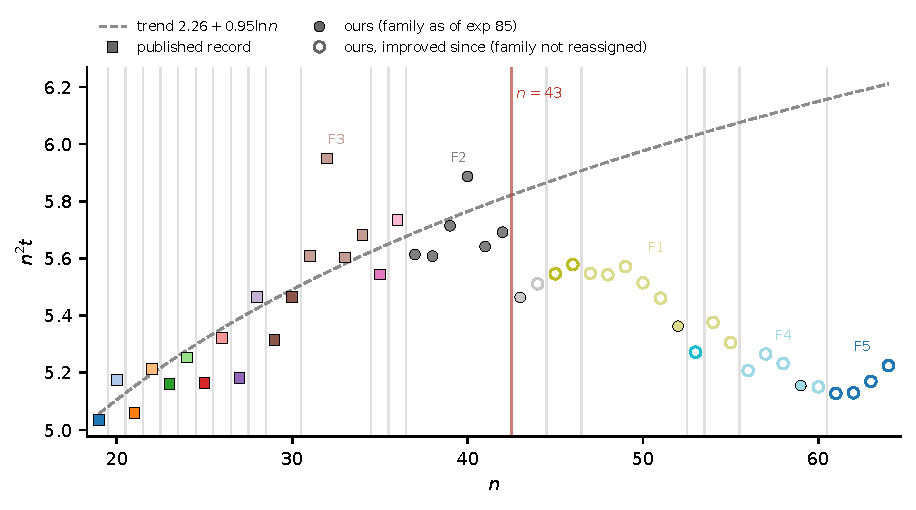
\includegraphics[width=0.88\linewidth]{fig_families.pdf}
  \caption{Best known $n^2t$ for $19 \le n \le 64$ in the current library (squares: published records; circles: ours; dashed: trend \eqref{eq:trend}), coloured by the family holding the best. Families and handovers (grey lines) are those of the family analysis, computed on the library of commit 091485f; open circles mark the 19 sizes ($44$--$51$, $53$--$58$, $60$--$64$) whose best has improved since, where the family label has not been recomputed.}
  \label{fig:families}
  % SRC: figures/make_paper_figures.py (exp 108); report_tex Sec. Phase 4 item 1 (Data)
\end{figure}

\subsection{Survival of minimal triangles}
After matching points across one growth step we measure the share of minimal triangles that survive. Within a family the median is $57$--$61\%$ (current-best and best-of-family pairs; descents $54$--$60\%$); at a handover $8$--$10\%$; between unrelated configurations $11\%$ (Figure~\ref{fig:survival}). For current-best pairs the within-vs-handover AUC is $0.99$ (Cohen's $d = 3.8$; best-pair version AUC $0.92$, $d = 2.5$). % SRC: experiments/101-red-team/NOTES.md (what checks out; issue 8)

\emph{Definitional bias.} Within-family survival is partly built into the descent-based definition: a descent deletes points and refines onto the member, which nearly implies shared minimal triangles. The informative contrasts are that handover pairs are as unrelated as random pairs ($8$--$10\%$ vs $11\%$), and the bias-free contrast below. % SRC: experiments/101-red-team/NOTES.md issue 8
Label-free definitions (tie overlap, affine share, plain geometry) agree with the descent families at adjusted Rand index $0.75$--$0.85$, against $0.73$ for a contiguous-block baseline; the sharper agreement is at window edges, where all 8 robust edges are found by every definition ($\approx 3.5$ expected by chance). % SRC: report_tex Sec. Phase 4 item 1 (exp 89)

\begin{figure}[htbp]
  \centering
  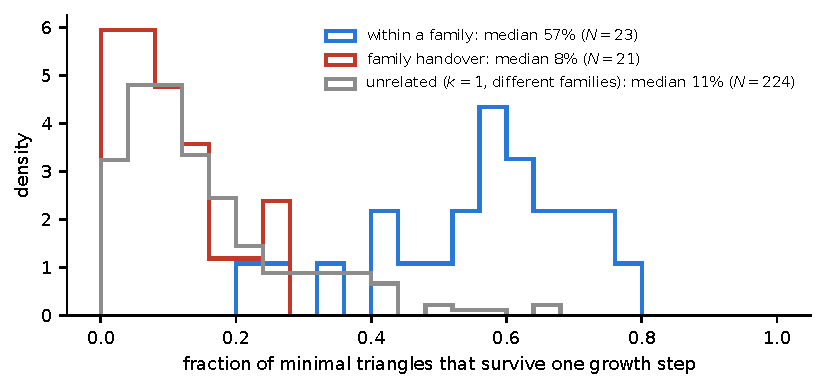
\includegraphics[width=0.88\linewidth]{fig_survival.pdf}
  \caption{Survival of minimal triangles across one growth step, for pairs of consecutive bests within a family (median $57\%$), at a handover ($8\%$), and for unrelated $k = 1$ pairs from different families ($11\%$); families and pairs as of library commit 091485f. Within-family survival is partly built into the family definition.}
  \label{fig:survival}
  % SRC: figures/make_paper_figures.py (exp 108; exp 85 pairs_survival.jsonl)
\end{figure}

\subsection{Is the skeleton a state variable?}\label{sec:skeleton}
We asked whether the set of minimal triangles (the \emph{skeleton}) carries information beyond geometry (our experiment~106; analysis on the best-per-$n$ sequences $20$--$64$ with 20 holder handovers and 8 robust edges). Tie survival alone detects every handover (AUC $0.93$ for holders, $0.85$ for robust edges; a label-free threshold finds 20 of 20 and 8 of 8). But plain non-affine point motion does as well (AUC $0.95$), the two correlate at Spearman $-0.92$, and with motion held fixed survival adds little (AUC $0.54$--$0.71$). In the one bias-free contrast (same family without descent vs cross-family pairs) survival is $0.38$ vs $0.12$, AUC $0.84$ (geometry alone $0.79$): a modest genuine skeleton signal. % SRC: STATUS.md row 106; report_tex Sec. Phase 5 item 4
Richer genealogies (one-vertex links, births, lineage depth) do worse than plain survival; stress-network spectra find only 7--8 of the 20 handovers and are blind to $n = 43$. About 18 scores were tried on two edge sets and two sequences; the AUCs and counts above are not corrected for this multiplicity, and the permutation nulls behind them treat handovers as exchangeable (they ignore autocorrelation). We conclude that the skeleton is a faithful readout of families, not a separate state variable. % SRC: STATUS.md row 106

\subsection{Growth inside a family}
Over all descents inside families, a single affine map removes $71\%$ of the point motion (null $27\%$, handovers $12\%$): a squeeze of about $1.5\%$ toward the wall where the new point lands ($79\%$ of new points land on a wall). For the container-free children of Section~\ref{sec:search} (a different population, parent to result) the fitted map is a $\sim4\%$ anisotropic shrink. % SRC: report_tex Sec. Phase 4 item 1 (exp 87); Innovations 6b; experiments/101-red-team/NOTES.md issue 17

% =====================================================================
\section{A crossover at \texorpdfstring{$n = 43$}{n = 43}}\label{sec:43}

We use the word \emph{crossover} for the combination of two statements, and we keep them apart from a third:
(a) a \emph{breakpoint in the measured best-known configurations}: observables of the best configuration per $n$ change jointly between $n = 42$ and $n = 43$ (Sections~\ref{sec:obs43}--\ref{sec:controls43});
(b) a \emph{change of best-known architecture}: below $43$ the best configurations we know have an empty centre, from $44$ on the best empty-centre configurations we can find are far below the filled-centre ones (Table~\ref{tab:emptycentre}).
Both are supported by our data, with the controls below. We do \emph{not} claim (c), a transition in the global optima: the configurations are best known, not optimal, and (b) is a search result.

\subsection{The observables}\label{sec:obs43}
Ten observables of the best configurations were tracked over $20 \le n \le 64$. One joint breakpoint at $n = 43$ explains them (model-based residual bootstrap $95\%$ interval $43$--$43$; a one-point interval reflects the step size, not independent replication), robust to even/odd splits, to using the top three instead of the best, to dropping any one observable, and to dropping any one family (control (b) below). % SRC: report_tex Sec. Phase 4 item 2 (exp 86)
It is carried by (Figure~\ref{fig:transition}):
\begin{itemize}
\item the central hole: with $\delta$ the distance from the centre to the nearest point, $2\delta\sqrt n = 1.22$--$2.41$ at $19$--$42$ and $0.33$--$0.81$ at $43$--$51$; it reopens to $0.93$--$1.35$ at $52$--$55$;
\item neighbours within $1.6/\sqrt n$, jumping from a mean of $4.05$ ($37$--$42$) to $5.19$ ($43$--$64$);
\item mean wall incidences, falling from $7.8$ ($37$--$42$) to $6.7$ ($43$--$64$); both ranges are $6$--$8$;
\item symmetry: every even best for $20 \le n \le 42$ has a symmetric core, and no best at $43$--$64$ is close to any symmetry of the square (RMS displacement under the nearest symmetry at least $0.015$, i.e.\ at least $0.108/\sqrt n$, against $0.02/\sqrt n$ for the symmetric bests of Figure~\ref{fig:phase}).
\end{itemize}
% SRC: experiments/101-red-team/NOTES.md issue 7 and (what checks out); report_tex Sec. Phase 4 item 2
$n^2t$ itself does not break: it peaks at $32$--$40$ and declines smoothly. There is no precursor: the symmetry-breaking stiffness shows no trend toward zero and the soft modes are symmetric, which points to a replacement of one architecture by another rather than a continuous instability of the best-known configurations. % SRC: report_tex Sec. Phase 4 item 2 (No precursor)

\begin{figure}[htbp]
  \centering
  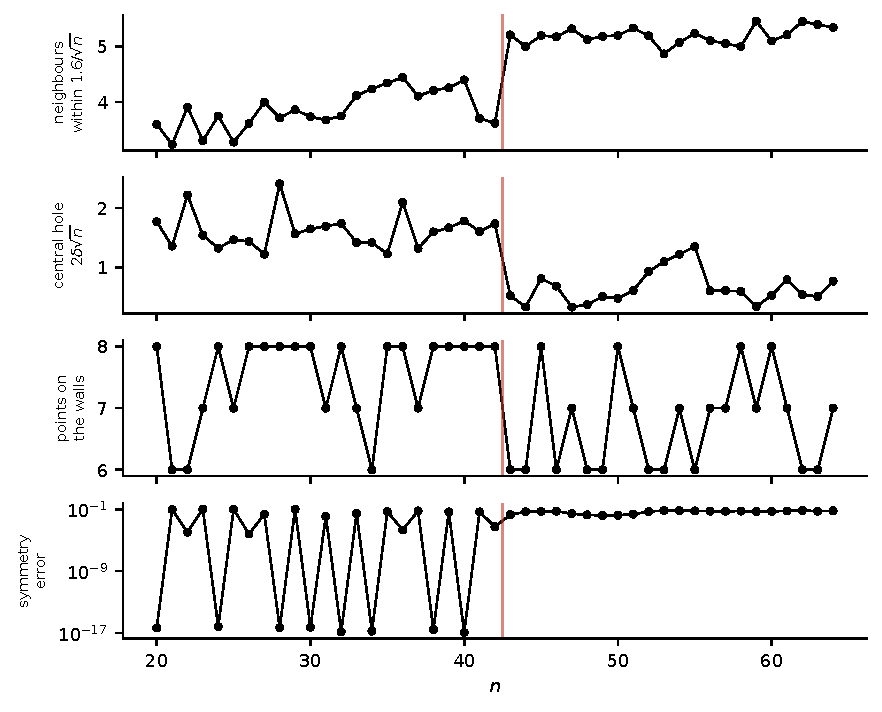
\includegraphics[width=0.88\linewidth]{fig_transition.pdf}
  \caption{Four of the ten observables, $n = 20$--$64$, recomputed on the current bests: neighbours within $1.6/\sqrt n$, central hole $2\delta\sqrt n$, points on the walls, symmetry error (RMS displacement under the nearest symmetry of the square). The joint breakpoint at $n = 43$ (vertical line) was fitted on the library of its run, which differs from the current one only at $n = 45, 46, 48$.}
  \label{fig:transition}
  % SRC: figures/make_paper_figures.py (exp 108; observables recomputed)
\end{figure}

\subsection{Controls and caveats}\label{sec:controls43}
\begin{enumerate}[label=(\alph*)]
\item \emph{Trend control.} Against smooth trends with AR(1) noise we simulate 300 null series and report $p = (1+k)/301$, where $k$ is the number of null draws whose statistic reaches the observed one. The structural joint statistic (gap, neighbours, layers) gives $p = 0.003$ ($k = 0$, the smallest value attainable with 300 draws) and the joint statistic over all observables $p = 0.007$; neither is corrected for the several statistics and windows tried. The null simulates each observable's noise independently although the observables co-move, and the observables were chosen after the change at $43$ had been noticed; both make $p$ optimistic. % SRC: experiments/101-red-team/NOTES.md issue 8; STATUS.md row 100
\item \emph{Leave one family out.} Families hold windows of consecutive sizes, so a single family could create the breakpoint. We dropped each of the 20 holders of the best (families and singletons of Section~\ref{sec:families}) in turn, with all of its sizes, and refitted the joint changepoint on its eight observables ($20 \le n \le 64$). It stays at $n = 43$ in every run except one: dropping the family that holds $43$ and $44$ leaves no size between $42$ and $45$, and the break moves to $45$, the first remaining size, i.e.\ to the same place. The bootstrap interval is a single point in every run, and the trend-control $p$ is $\le 0.017$ in every run ($0.003$--$0.017$; permutation $p = 0.020$, the floor for 50 permutations). So the breakpoint is not produced by any single family; the caveats of (a) apply to each run. % SRC: experiments/109-loo-family/NOTES.md (loo.json, loo.log); STATUS.md row 109
\item \emph{A search with the hole as a hard constraint} (Table~\ref{tab:emptycentre}). Calibrated at $40$--$42$, where it lands $0$--$1.8$ points of trend below the known empty-centre bests, it stays far below the filled-centre bests from $n = 44$. % SRC: report_tex Sec. Phase 4 item 2 table (exp 88)
\item \emph{The calibration does not transfer.} At $40$--$42$ it starts from $n-1$ members of the known empty-centre family; at $44$ and beyond no good empty-centre seed exists. Our one-rung growth controls elsewhere miss known optima by $10$--$30$ points (the $40$ family grown to $44$ lands at $-10.6\%$; $28 \to 30$ lands at $-17$ to $-23\%$ against $-0.47\%$; $40 \to 42$ at $-12$ to $-30\%$ against $-2.05\%$). So $0$--$1.8$ points does not bound the error at $44$--$50$. % SRC: experiments/101-red-team/NOTES.md issue 1
\item \emph{A prediction test} (``at least 10 points below at $47$--$50$'') was met at $48$ and $50$ and narrowly missed at $47$ and $49$ ($9.0$, $9.7$). A weaker search can only enlarge the gap, so this is weak evidence. % SRC: experiments/101-red-team/NOTES.md issue 1
\end{enumerate}

\begin{table}[htbp]
\centering\small
\caption{Empty-centre search vs the library (percent of trend). ``Hole kept'': the hole imposed as a constraint; ``released'': after removing it (centre gap $2\delta\sqrt n$ in parentheses).}\label{tab:emptycentre}
% SRC: report_tex/heilbronn_report.tex Sec. Phase 4 item 2 table (exp 88; library values current)
\begin{tabular}{@{}lllll@{}}
\toprule
$n$ & hole kept & released (gap) & library & gap to library \\
\midrule
43 & $-7.68$ & $-7.04$ (1.61) & $-6.34$ & 0.7 \\
44 & $-12.36$ & $-12.29$ (1.18) & $-5.87$ & 6.5 / 6.4 \\
45 & $-13.74$ & $-13.52$ (0.96) & $-5.62$ & 8.1 / 7.9 \\
46 & $-13.13$ & $-12.84$ (1.06) & $-5.41$ & 7.7 / 7.4 \\
47--50 & $-15.2$ to $-20.1$ & about the same (1.19--1.38) & $-6.2$ to $-7.7$ & 9.0--12.3 \\
\bottomrule
\end{tabular}
\end{table}

Tripling the budget, a smaller hole and symmetric seeds grown from the $40/42$ family did not close the gap. Our reading: for $n \le 42$ every best configuration we know has an empty centre; at $n = 43$ the best empty-centre configuration we found is within $0.7$ points of trend of the best filled-centre one; from $n = 44$ a search aimed at empty-centre configurations stays $6.4$--$8.1$ points below at $44$--$46$ and $9$--$12$ points below at $47$--$50$. This is strong evidence of a change of best-known architecture (statement (b)), but it is a search result, and it says nothing about the global optima. % SRC: report_tex Sec. Phase 4 item 2 (Reading); experiments/101-red-team/NOTES.md issue 1
At small $n$ no best-known configuration for $5 \le n \le 42$ (proved optimal for $n \le 8$, and for $n = 9$ by the computer-assisted proof of \cite{N9}) has a central point; the gap stays $\ge 1.05$, thinnest at $n = 18$ ($1.05$), $11$ ($1.17$) and $7$ ($1.21$). % SRC: STATUS.md row 102; report_tex Sec. Phase 4 item 6

\subsection{Why 43? What was rejected}
\begin{itemize}
\item \emph{Ring capacity.} $k$ points on a circle of radius $R$ have minimal triangle $2R^2\sin^2(\pi/k)\sin(2\pi/k)$; the real rings sit at about half that capacity at every $n$, and their minimal triangles are long ($\sim0.7$ of the side). % SRC: report_tex Sec. Phase 4 item 3
\item \emph{Wall pattern.} Forcing two points per edge costs $0.1$--$1.3$ points of trend, against $6$--$12$ for forcing the hole. % SRC: report_tex Sec. Phase 4 item 3
\item \emph{Symmetry.} Lemma~\ref{lem:group}(a) is true but limited (8 of 24 sizes, and only a gap of order $t$).
\item \emph{Idealised two-core models} did not derive the switch. % SRC: report_tex Sec. Running now (exp 97)
\item \emph{Half-turn symmetry of the region.} Our earlier hypothesis that the empty centre comes from the half-turn symmetry of the square and of its inherited symmetric families is refuted by the regular pentagon, which has no half-turn and still has an empty centre at $13 \le n \le 20$ (Section~\ref{sec:halfturn}). % SRC: STATUS.md row 107
\end{itemize}

\subsection{A surviving candidate: the closed band}
The empty-centre core inherited from the symmetric $40/42$ has convex layers $[10,4,6]$ and a nearly centrally symmetric inner hexagon. Inserting a centre point costs $26$--$41$ points of trend, against $5$--$17$ for a point in the band between the layers. At $41$--$42$ its outer ring comes within $\sim0.48$ spacings of all four walls (filled core: $1.27$), which splits the band into four corner pockets. Growth confined to a fixed region of $m$ points costs $t \propto m^{-2}$: predicted $-4.2$ points of trend per added point, measured $-5.1$, against about $-1.2$ for the filled architecture. The ratio $\approx 4.25$ splits into $1.75$ (band size, derived) and $2.4$ (closure, measured). The two value curves cross at $n \approx 42.8$, but only with the slopes at $41$--$46$ as input. We regard the closed band as a candidate mechanism with moderate evidence (two or three growth steps); the location of the switch is not derived from first principles. % SRC: report_tex Sec. Phase 4 item 3 (exp 92)
Figure~\ref{fig:phase} shows that the centre is empty at every $n \le 42$ across 3, 4 and 5 convex layers, so the layer count does not drive the switch. % SRC: report_tex Sec. Phase 4 item 3 (phase diagram)

\begin{figure}[htbp]
  \centering
  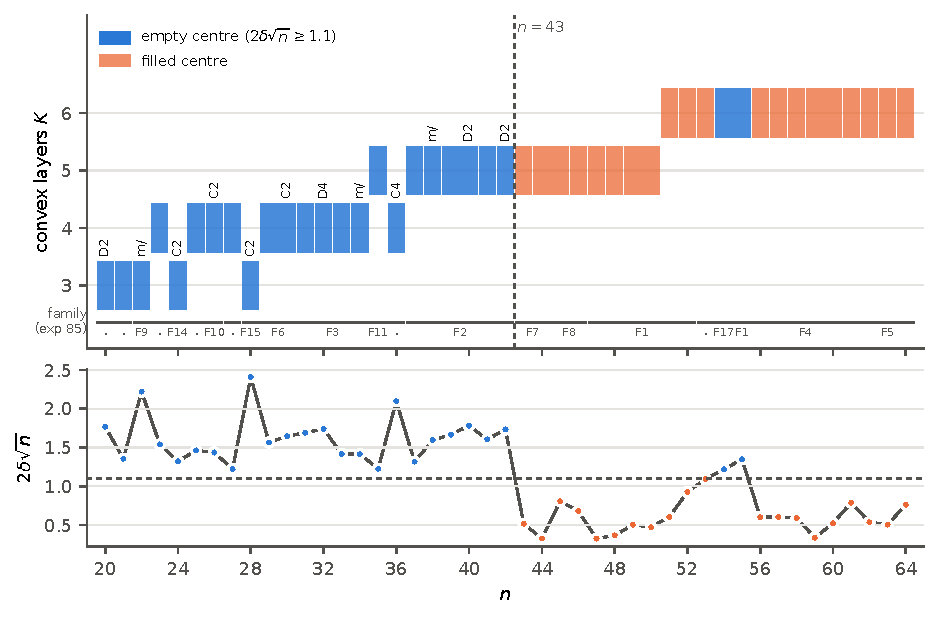
\includegraphics[width=0.95\linewidth]{fig_phase.pdf}
  \caption{Phase diagram of the current best configurations, $n = 20$--$64$. Top: number of convex layers, coloured by empty ($2\delta\sqrt n \ge 1.1$, blue) or filled (orange) centre, with the symmetry group above each tile (RMS displacement $< 0.02/\sqrt n$); family brackets as in Figure~\ref{fig:families} (library commit 091485f; dot: singleton). Bottom: centre gap $2\delta\sqrt n$. The centre is empty for $n \le 42$ and at $54, 55$.}
  \label{fig:phase}
  % SRC: figures/make_paper_figures.py (exp 108; exp 92 definitions)
\end{figure}

\subsection{A physical analogue}
In two-dimensional confined charged clusters a central particle appears when the inner ring fills \cite{BP}. The analogy offers a reading of the brief reopening of the centre at $52$--$55$ (cycling of the innermost shell). It does not locate $43$: Coulomb clusters in a square change centre occupancy $8$--$11$ times over the same range (ours: $3$), because their walls hold $60$--$90\%$ of the particles and ours at most $8$ points. % SRC: report_tex Sec. Phase 4 item 3 (exp 96) % CHECK: cluster numbers come from our own simulation (exp 96), not from [BP]

\subsection{No robust second breakpoint up to \texorpdfstring{$n = 100$}{n = 100}}
A first pass over $65$--$100$ suggested a joint break near $n \approx 75$. Rebuilding $60$--$100$ in an independent second lineage, the joint break fails the same trend control in every library: first pass $p = 0.29$, lineage A $p = 0.28$, lineage B $p = 0.36$, combined $p = 0.12$. At most a weak, lineage-dependent closing of the centre remains (lineage A at $73$, B at $71$; none in the combined library). Layer changes beyond $64$ also depend on the lineage ($6\to7$ at $68$--$70$, $7\to8$ at $74$--$80$, $8\to9$ at $89$--$91$). So $n = 43$ is the only robust breakpoint we found in $20 \le n \le 100$. % SRC: STATUS.md row 100; report_tex Sec. Phase 4 items 3, 5

% =====================================================================
\section{Small \texorpdfstring{$n$}{n}}\label{sec:smalln}

\subsection{The laws on proven optima}
With the configurations for $5 \le n \le 18$ rebuilt by our own search (Section~\ref{sec:search}) and the records $19$--$36$, we tested the laws above where optima are proven ($5$--$9$), optimal within solver tolerances ($10$ \cite{SM}) or long-standing records. No law fails on the proven optima. Interleaving holds at every certified strict maximum (including $n = 5, 7, 8, 9$); the $n = 6$ shear family is not strictly interleaved, as Theorem~\ref{thm:interleave} allows for a non-strict maximum. As stored, the $2n-7$ bound holds for $5 \le n \le 21$ (with equality at $9$, $17$, $19$, and later at $27$; since rattlers can be moved without changing $f$, the count of a configuration depends on where its rattlers sit, e.g.\ record $21$ can be brought down to $33 < 35$, which is why the existential reading matters \cite{Note2}), and the tie counts for $5 \le n \le 16$ equal Sudermann-Merx's table \cite[Table~10]{SM}. Every half-turn-symmetric configuration among them is even without a centre point; every odd one is $C_1$ or a single mirror. Trela's statements (equal side forces; a single stress component touching all four sides) hold on all 44 configurations examined. No rattlers occur for $n \le 20$. % SRC: STATUS.md row 102; report_tex Sec. Phase 4 item 6
Besides the known shear family at $n = 6$, our runs found the four corners together with $(\tfrac12,\tfrac14)$ and $(\tfrac12,\tfrac34)$, with value exactly $1/8$, $10$ minimal triangles and symmetry $D_2$, certified as a strict local maximum. We have not checked it against \cite{DYZ}; it may well be classical, and we do not claim it. % SRC: STATUS.md row 102 % CHECK against Dress--Yang--Zeng

\subsection{Rigorous proofs for \texorpdfstring{$n = 7$, $8$ and $9$}{n = 7, 8 and 9}}
These optima are known \cite{ZC,DZ}; we give an independent computer proof (our experiment~103). % SRC: STATUS.md row 103; report_tex Sec. Phase 5 item 1
\emph{Method.} Branch and bound over boxes of point positions on a grid of $2^{-24}$, after exact reductions (ordering of points, stretching to touch all four walls, two mirrors). A box is discarded if some triple has $\lvert\Delta\rvert \le T$ at every corner tuple (checked exactly), or if a McCormick LP relaxation bounds the minimum area by $T$. The LP only proposes multipliers; they are rounded to integers and the bound is re-derived in exact integer arithmetic. Boxes inside the certified basin ball of Section~\ref{sec:cert} around the optimum are covered by that local theorem.
\emph{Soundness.} Floating point only chooses splits, duals and point matchings; a wrong choice costs time, not soundness. A box that can be neither split nor discarded is reported as a failure; both runs had none. We also ran a randomised soundness test, an audit mode re-deriving the LP certificates with rational arithmetic, and a negative control that fails as it should. The trusted base is about 500 lines of Python plus the certifier of Section~\ref{sec:cert}; neither is formally verified.
\emph{Result.} Every configuration with minimum area $> t^*(1-10^{-9})$ lies within sup distance $2.1\cdot10^{-4}$ ($n = 7$) or $1.37\cdot10^{-4}$ ($n = 8$) of a symmetric copy of the certified optimum; hence the global maximum is $t^*$, attained uniquely up to the symmetries of the square. The runs took $1.17$ million nodes and 73 minutes on one core ($n = 7$), and $4.26$ million nodes and $3.5$ core-hours ($n = 8$). For $n = 5, 6$ the method gives only $H(n) \le t^*(1+10^{-3})$, since $n = 5$ is second order and $n = 6$ a family, so no basin ball exists.
\emph{$n = 9$.} A sped-up version of the same method (warm-started LPs, compiled node code, an additional symmetry cut; experiment~110) proves that every configuration of $9$ points in the square has minimum area at most $t^* = (9\sqrt{65}-55)/320 = 0.0548759991\ldots$, with equality only at the known configuration up to the symmetries of the square. The run closed $358.6$ million boxes in $16$ hours on $14$ workers with no failures; $21\,286$ LP certificates were re-derived in rational arithmetic as an audit, and the code was first re-validated on $n = 7, 8$. (The random-probe estimate had been $3\cdot10^8$ nodes.) If correct, this settles the value that Chen, Xu and Zeng \cite{Chen17} bracketed and that Sudermann-Merx \cite{SM} and Monji, Modir and Kocuk \cite{MMK} found optimal within solver tolerances; the proof is computer- and AI-assisted, has not yet been independently checked, and is presented in the companion paper \cite{N9}. $n = 10$ needs a stronger local certificate. % SRC: experiments/110-n9-proof/NOTES.md (Result); STATUS.md rows 103, 110

\subsection{Exact values}
High-precision Newton iteration (up to 8000 digits), LLL to guess a minimal polynomial, an exact check in $\Q[x]/(p)$ and a Krawczyk uniqueness test give exact values for 12 configurations at 11 sizes (Table~\ref{tab:exact}). % SRC: STATUS.md row 104; report_tex Sec. Phase 5 item 2
``Proved'' means: there is an exact configuration with coordinates in $\Q(t)$, within about $10^{-13}$ of the record, whose minimum area is exactly the stated root, and it is the unique solution of the active system near the record. That this is the record's value rests on the site's floating-point coordinates agreeing to $\le 10^{-13}$; local optimality is the subject of Section~\ref{sec:cert} where a certificate exists (record $20$ has none), and global optimality is known only for $5 \le n \le 9$ ($n = 9$ by \cite{N9}). % SRC: report_tex Sec. Phase 5 item 2

\begin{table}[htbp]
\centering\small
\renewcommand{\arraystretch}{1.2}
\caption{Exact values of the best-known square configurations. Known values: $5$--$11$, $16$ \cite{SM,CY}; $12$ is in Comellas--Yebra \cite{CY}; $14$ is on the record site (Chappell \cite{Chappell}); $20$ was not found in the literature we read (the record site's $n = 20$ page gives a different, degree-20 polynomial, which the record value does not satisfy).}\label{tab:exact}
% SRC: report_tex/heilbronn_report.tex Sec. Phase 5 item 2 table; STATUS.md row 104
\begin{tabular}{@{}rll@{}}
\toprule
$n$ & minimal polynomial of $t$ & closed form \\
\midrule
5 & $27x^2-1$ & $\sqrt3/9$ \\
6 & $8x-1$ (shear family and the $D_2$ optimum) & $1/8$ \\
7 & $152x^3+12x^2-14x+1$ & trigonometric form (real cubic) \\
8 & $108x^2+6x-1$ & $(\sqrt{13}-1)/36$ \\
9 & $320x^2+110x-7$ & $(9\sqrt{65}-55)/320$ \\
10 & $3456x^3-1764x^2+268x-9$ & Cardano form \\
11 & $27x-1$ & $1/27$ \\
12 & $64x^3+80x^2+28x-1$ & $\bigl(\sqrt[3]{46+6\sqrt{57}}+\sqrt[3]{46-6\sqrt{57}}-5\bigr)/12$ \\
14 & $320x^3+768x^2-60x+1$ & trigonometric form (real cubic) \\
16 & $341x-7$ & $7/341$ \\
20 & degree 19, leading coefficient $3\cdot2^{42}$ & none: Galois group $S_{19}$ \\
\bottomrule
\end{tabular}
\end{table}

For $n = 10$ the value is $\bigl(49 - \sqrt[3]{8831 + 992\sqrt{62}} - \sqrt[3]{8831 - 992\sqrt{62}}\bigr)/288$; the trigonometric forms for $7$ and $14$ are given in our data. % SRC: report_tex Sec. Phase 5 item 2 table
At $n = 20$ the Galois group is $S_{19}$, proved from factorisation patterns modulo primes (modulo $349$ the pattern yields a transposition); hence $t(20)$ has no expression in radicals. % SRC: report_tex Sec. Phase 5 item 2
No polynomial was found for $13, 15, 17, 18$ up to degree $200$, for $19, 21$--$27$ up to $150$, or for $28$--$36$ up to $70$ (with moderate coefficients); these are search bounds, not proofs of high degree. Apart from the rational values at $n = 6, 11, 16$, no two sizes share a field $\Q(t)$; low degree occurs only at symmetric sizes (except $n = 7$), but symmetry is not sufficient. % SRC: STATUS.md row 104
\emph{Caveat at $n = 24$.} The record site's methods page credits Chappell with ``the degree-15 exact value for square $n = 24$''; neither the $n = 24$ page (which credits the configuration to Sudermann-Merx, October 2026) nor the leaderboard prints it (checked 12 November 2026), our search found no relation up to degree 150, and our polished value is $2.6\cdot10^{-12}$ (relative) above the site's literal. This conflict is unresolved. (The site states that contributed polynomials are checked to 45 digits against its literal value, which differs from our polished value in the twelfth significant digit.) Similarly, the site's $n = 20$ record history (2026-09-15) identifies the value as the smallest positive root, $0.0129115556839\ldots$, of an irreducible degree-20 polynomial with leading coefficient $2^{22}\cdot3^4\cdot7\cdot97^2\cdot15185077^2$; the record value $0.0129381967\ldots$ is not a root of it, whereas it is a root of our degree-19 polynomial, and the two polynomials are coprime. The site's root agrees to 16 digits with the value of a different $n = 20$ configuration in our library ($0.2\%$ below the record), so the history entry appears to describe an earlier configuration, not the current record. % SRC: STATUS.md row 104; experiments/LITERATURE.md (arXiv sweep) % CHECK with the site / Chappell

% =====================================================================
\section{Other regions}\label{sec:regions}

\subsection{Triangle and convex-hull variant}
We ported the engine to a triangle ($6 \le n \le 30$; optimal for $n \le 8$ by \cite{SMtri}) and to the record site's convex-hull variant (value $=$ minimum area / hull area, $6 \le n \le 20$). The triangle records were matched at $n = 6$--$15$, $18$ and $24$ without the site's coordinates; triangle $27$--$30$ are still $12$--$17\%$ below the records, so structural statements there describe our configurations, not the records. The convex records were matched at $6$--$16$ and $18$. % SRC: STATUS.md row 105; report_tex Sec. Phase 5 item 3
\begin{itemize}
\item \emph{Universal:} the wall-force law (Theorem~\ref{thm:polygon}; 25 of 25 triangle bests), Trela-type statements (a single stress component touching all sides) and the rank--nullity count, whose natural form is $2n+1-(\text{maximal number of loaded walls})-d$: $2n-5$ in the triangle (at most 6 loaded walls) and also $2n-5$ in the convex variant (no walls, but a 6-dimensional affine gauge). % SRC: STATUS.md row 105
\item \emph{Square-specific:} the stored count is below $2n-7$ at the triangle record $n = 15$ and at the convex $n = 7$; $d \le 1$ fails at triangle $15$ ($d = 4$) and at convex $7, 9, 13, 14$ ($d = 2$--$3$). These $d$ values are first-order counts at optima that may be non-isolated, so they do not contradict Observation~\ref{obs:dof}. % SRC: STATUS.md row 105; experiments/105-shape-universality/NOTES.md
\item \emph{No empty centre and no switch in the triangle:} bests have centre points at $7$, $16$, $22$, and there is no change point ($p = 0.98$ against a line + AR(1) null). The convex variant has an empty centre at $10$--$20$, with a gap that grows smoothly. % SRC: STATUS.md row 105
\end{itemize}

\subsection{Half-turn test (hexagon vs pentagon)}\label{sec:halfturn}
% Filled from STATUS.md row 107 and experiments/107-half-turn-test/NOTES.md (exp 107 completed 2026-11-12).
After the triangle results we proposed that the square's empty centre comes from the half-turn symmetry of the region; the prediction was an empty-centre phase in a regular hexagon (which has a half-turn) and none in a regular pentagon (which has none). We tested this on the regular hexagon and pentagon ($8 \le n \le 30$) and the disk ($10 \le n \le 26$, exact disk constraint), all of area 1, with the same engine. % SRC: experiments/107-half-turn-test/NOTES.md (Hypothesis, Method)
With $\delta$ the distance from the centroid to the nearest point and the gap $2\delta\sqrt n$, the block means (gap / void percentile, the share of test points in the central zone whose own void is smaller than the centre's) are:
\begin{center}\small
% SRC: experiments/107-half-turn-test/NOTES.md (Block means)
\begin{tabular}{@{}llll@{}}
\toprule
region & $8$--$12$ & $13$--$20$ & $21$--$30$ \\
\midrule
hexagon (half-turn) & $1.15$ / $0.54$ & $1.76$ / $0.97$ & $2.16$ / $0.78$ \\
pentagon (none) & $0.97$ / $0.53$ & $1.54$ / $0.85$ & $1.19$ / $0.36$ \\
disk (half-turn) & $0.94$ / $0.58$ & $1.88$ / $0.98$ & $0.98$ / $0.27$ ($21$--$26$) \\
\bottomrule
\end{tabular}
\end{center}
\begin{itemize}
\item \emph{The prediction fails.} At $13 \le n \le 20$ all three regions have an empty centre, including the pentagon. So the empty centre at these sizes is not a half-turn effect; among the regions tested the triangle is the exception, not the rule. Possible causes (the triangle's sharp corners and small inradius, or its $C_3$ arithmetic forcing centre points at $n \equiv 1 \pmod 3$) were not tested. % SRC: experiments/107-half-turn-test/NOTES.md (Verdict)
\item At $21 \le n \le 30$ the hexagon stays empty (its one centre point, at $n = 25$, is forced by $C_3$ symmetry), while the pentagon and the disk begin to fill. The disk has a half-turn, so this split does not follow half-turn symmetry either. No series has a significant change point (hexagon $p = 0.80$, pentagon $0.95$, disk $0.73$), and the searches at $n \ge 21$ are not converged (mostly one hit per size), so we regard this range as ambiguous. % SRC: experiments/107-half-turn-test/NOTES.md (Results, Search quality)
\item Lemma~\ref{lem:group} holds in every case: hexagon $25$ is $C_3$ with a centre point, pentagon $21$ is $C_5$ with a centre point, pentagon $20$ and $25$ ($D_5$, $C_5$, $n \equiv 0$) have none, and disk $22$ is $D_7$ with a centre point. % SRC: experiments/107-half-turn-test/NOTES.md (Group arithmetic)
\item The wall-force law holds at all 63 bests (Theorem~\ref{thm:polygon}(b)); minimal-triangle counts fall below $2n-7$ in every region (hexagon $17, 20, 23, 26, 28, 30$; pentagon $8, 13, 17, 19, 30$; disk $10, 11, 14, 22, 26$). % SRC: experiments/107-half-turn-test/NOTES.md (Wall law)
\end{itemize}
Searches are converged only for $n \le 12$ (3--9 independent hits), so all readings beyond that are provisional. Why the square fills its centre at $n = 43$ remains open. % SRC: STATUS.md row 107

% =====================================================================
\section{Negative results}\label{sec:negative}
For the record, the following did not work (each documented in our data).
\begin{itemize}
\item \emph{Same-$n$ moves:} tie edits and pivots, ruin-and-recreate, stress-guided deletion, soft deletion, a smoothed minimum, morphing, grow-hop-prune, edge slides. Good optima are isolated at fixed $n$: eight families of same-$n$ moves return to the seed, and from-scratch methods fail above $n \approx 28$. % SRC: report_tex Sec. Innovations (Ideas tested and closed); Sec. What we found item 11
\item \emph{Starts and schemes:} random, greedy, ring, lattice and conic starts; population ladders, genetic algorithms, longer hops, large growth steps; an AlphaEvolve-evolved program above $n = 28$; population basin hopping (no better than ordinary kicks at equal time). % SRC: report_tex Sec. Innovations (Ideas tested and closed); STATUS.md row 100
\item \emph{Structure-based ideas:} symmetric orbit growth; Fourier, algebraic-modular, lattice and motif seeds; hypercube and Minkowski constructions beyond $n = 16$. A 74-descriptor motif atlas over 408 configurations found no hidden algebraic or lattice structure. % SRC: report_tex Sec. Phase 3 (Closed); What we found item 7
\item \emph{Collective deformations:} per-axis warps, tapered shifts, affine squeezes and shears; projective kicks and square--quadrilateral--square continuation (every path returns to its start); non-affine domain unfolding. % SRC: report_tex Sec. Innovations (Ideas tested and closed); Phase 3 (Closed)
\item \emph{Recombination and insertion:} an exact MILP recombination of elites; weighted constraint-release insertion; stress-weighted insertion scores (no better than the plain hole score). % SRC: report_tex Sec. Phase 2 (exp 60), Phase 3 (Closed)
\item \emph{Symmetry:} symmetrising configurations far from symmetric; a symmetric growth ladder; growing the $n = 40$ with symmetric point groups ($42$--$48$ land $11$--$20\%$ below our library). % SRC: report_tex Sec. 5c, Phase 3 (Closed)
\item \emph{Global certificates:} the stress matrix has balanced inertia at all 127 configurations tested, so universal-rigidity-type certificates cannot prove optimality here; interval/MINLP upper bounds were not feasible at $n \ge 20$. % SRC: report_tex Sec. Phase 4 item 4; Innovations (Bounds)
\end{itemize}

% =====================================================================
\section{Discussion and open problems}\label{sec:open}
The configurations studied here are best known, not optimal; every structural statement is about them, and those beyond $n \approx 45$ are probably far from optimal. The theorems of Section~\ref{sec:theory} are elementary consequences of affine invariance and Trela's identity, and their role is to organise the data and to filter certificates.
\begin{enumerate}[label=(\arabic*)]
\item \emph{Why $43$?} Derive the location of the switch from first principles. The closed-band picture gives the slopes but needs one measured anchor; the half-turn explanation is refuted (Section~\ref{sec:halfturn}).
\item \emph{Does the crossover at $43$ reflect the optima?} A stronger empty-centre search at $44$--$50$, or a proof that empty-centre configurations are bounded away from the filled ones, would turn the change of best-known architecture into a statement about optima.
\item \emph{Is $d \le 1$ at isolated square optima a theorem?} It holds at every certified best but fails in other regions (at possibly non-isolated optima).
\item \emph{Can $n = 10$ be proved optimal} with a sound branch and bound? The $n = 9$ proof \cite{N9} does not extend directly: it needs a stronger local certificate.
\item \emph{Exact forms:} are the values for $13, 15, 17$--$19$ and $21$--$36$ of very high degree? Do symmetric sizes in $37$--$64$ have low degree?
\item \emph{Large $n$:} is the decline of $n^2t$ beyond $42$ a property of the problem or of the search?
\item \emph{Critical triangles:} under the existential reading no record ($5 \le n \le 36$) contradicts the $2n-7$ conjecture, while the universal reading fails at record $22$ if that record is optimal; does it hold for optima, and is $2n+1-w-d$ after rattler repair the right general count \cite{Note2}?
\end{enumerate}

\subsection{A mechanical interpretation}\label{sec:mech}
The KKT conditions of Section~\ref{sec:methods} have a mechanical reading, which organises the results above; it adds no new claims. View a configuration at a KKT pair as a weighted hypergraph on its points. Each loaded tie $T$ is a hyperedge on three points with weight $\lambda_T > 0$ (the weights sum to $1$), and it pulls on its vertices with forces $\lambda_T\nabla_{p}(\sigma_T\Delta_T)$; each loaded wall contact $c$ is a boundary reaction $\mu_c a_c$. Stationarity says that every core point is in equilibrium under these forces, and rattlers are the points that carry no force.
\begin{itemize}
\item \emph{Global equilibrium.} Contracting the point equilibria with affine velocity fields gives \eqref{eq:virial}: the reactions balance as a whole, each side of the square carries total force $t$ and opposite sides have equal moments (Trela's identity, Proposition~\ref{prop:trela}). The polygon law (Theorem~\ref{thm:polygon}) is the same statement for other containers; in a triangle it fixes every side force and centroid.
\item \emph{Flat directions.} $\ker J$ consists of the first-order motions that keep every loaded constraint at its value: mechanisms of the hypergraph. Its dimension $d$ is the number of flat directions, and at a second-order maximum the Lagrangian Hessian plays the role of a stiffness on them. Proposition~\ref{prop:dof} is the Maxwell-type count of constraints against degrees of freedom. Its tightness at 36 of 44 sizes says that the best configurations are, in this sense, nearly isostatic: they carry almost no redundant constraints. The excess at the symmetric sizes corresponds to non-unique multipliers, i.e.\ self-stresses.
\item \emph{Families and the crossover.} In this language a family is a hypergraph that persists, with small changes, under growth (median survival of minimal triangles $57$--$61\%$ within a family, $8$--$10\%$ at a handover), and a handover replaces one hypergraph by another. The crossover at $43$ is such a replacement, between an empty-centre and a filled-centre architecture.
\end{itemize}
The reading has a clear limit. In our experiment~106 (Section~\ref{sec:skeleton}) the observables built from the hypergraph track family identity: tie survival finds every handover, but it is matched by plain point motion. The stress-network spectra find only 7--8 of the 20 handovers, and none of these observables sees $n = 43$. A later test (experiment~111) of stress concentration ($\sum\lambda_T^2$), a Jacobian rigidity ratio, the wall share of the stress and the spread of point loads over $20 \le n \le 64$ was also negative: after the same trend control none of them breaks at $43$. So the mechanical picture describes the families, but it does not yet explain the crossover. Left open are the spectrum of the Lagrangian Hessian on the tangent space (beyond the balanced inertia of the stress matrix noted in Section~\ref{sec:negative}) and insertion penalties (the cost of adding a point to a stressed region; compare the measured costs of a centre point and of a band point in Section~\ref{sec:43}). % SRC: STATUS.md row 106; experiments/101-red-team/NOTES.md issue 2; report_tex Sec. Phase 4 items 1, 3, 4


% =====================================================================
\appendix
\section{The published records \texorpdfstring{$19 \le n \le 36$}{19 <= n <= 36}: reproduction check}\label{app:records}
Table~\ref{tab:records} lists the records of \cite{Stead} used as calibration, with how our search reached the record value: \emph{own} (from our own structures), \emph{neighbour} (by growing or shrinking a neighbouring published record) or \emph{check} (only by shrinking the record and regrowing it). ``Best distinct'' is our best configuration sharing fewer than half of its points with the record. Records $21$--$36$ are certified local maxima by both codes of Section~\ref{sec:cert} where applicable ($16$ of $16$ by experiment~44); record $20$ has no certificate. % SRC: report_tex/heilbronn_report.tex Sec. Status 19-36; experiments/101-red-team/NOTES.md (certificates 16/16; record 20 no certificate)

\begin{table}[htbp]
\centering\small
\caption{Records $19 \le n \le 36$ \cite{Stead} and our reproduction. At $n = 33$ the route is from a log; coordinates were not kept.}\label{tab:records}
% SRC: report_tex/heilbronn_report.tex Sec. Status of every n (19-36 table)
\begin{tabular}{@{}rrrlr@{}}
\toprule
$n$ & record $t$ & $n^2t$ & reached & best distinct \\
\midrule
19 & 0.01394786 & 5.035 & own & $-4.03\%$ \\
20 & 0.01293820 & 5.175 & own & $-0.21\%$ \\
21 & 0.01147376 & 5.060 & own & $-1.86\%$ \\
22 & 0.01077166 & 5.213 & own & $-1.96\%$ \\
23 & 0.00975729 & 5.162 & check & $-1.17\%$ \\
24 & 0.00912014 & 5.253 & check & $-0.60\%$ \\
25 & 0.00826159 & 5.163 & check & $-1.06\%$ \\
26 & 0.00787271 & 5.322 & check & $-4.34\%$ \\
27 & 0.00710671 & 5.181 & check & $-0.48\%$ \\
28 & 0.00697109 & 5.465 & own & $-1.01\%$ \\
29 & 0.00631890 & 5.314 & neighbour & $-1.30\%$ \\
30 & 0.00607242 & 5.465 & neighbour & $-0.56\%$ \\
31 & 0.00583707 & 5.609 & neighbour & $-6.45\%$ \\
32 & 0.00581090 & 5.950 & own & $-6.19\%$ \\
33 & 0.00514549 & 5.603 & neighbour & $-1.72\%$ \\
34 & 0.00491472 & 5.681 & neighbour & $-1.62\%$ \\
35 & 0.00452533 & 5.544 & neighbour & $-0.33\%$ \\
36 & 0.00442536 & 5.735 & check & $-4.39\%$ \\
\bottomrule
\end{tabular}
\end{table}

Record $34$ was reached from record $32$ by shift-insert followed by refinement alone; this is the case the move was designed from, so it is an in-sample result. Among the records, the growth steps that keep or fill wall slots ($29 \to 30$, $31 \to 32$) are rigid nestings (the smaller configuration sits inside the larger to within $0.02$), while those that empty a slot ($32 \to 33$, $32 \to 34$, $33 \to 34$) displace every point by $0.02$--$0.06$. Out of sample (69 reconstructed growth steps at $37$--$64$) only the one-way statement survives: every displaced step emptied a wall slot ($3$ of $3$, against $0$ of $47$ keep-or-fill steps; one-sided Fisher exact test $p \approx 0.03$, uncorrected). % SRC: report_tex Sec. Innovations item 1; Sec. The transition framework; experiments/101-red-team/NOTES.md (Fisher p check)

\section{The shear-sign condition}\label{app:shear}
For completeness we record the first-order statement behind Theorem~\ref{thm:interleave} for local maxima that need not be strict. % SRC: experiments/99-wall-contact-bound/NOTES.md Thm 1(i)
\begin{proposition}
Let $P$ be a local maximum with $f(P) > 0$. Then on each pair of opposite walls both walls are touched and the ranges of contact coordinates intersect. If both pairs are only weakly separated, at $y = y_0$ and $x = x_0$ respectively, and the admissible shears $\ell = c(y - y_0)$ and $m = b(x - x_0)$ allow signs with $c\, b < 0$, then $P$ is not a local maximum.
\end{proposition}
\begin{proof}
If a pair is strictly separated (or a wall is empty), Lemma~\ref{lem:pair}(a) gives an admissible direction with $\tr A = a > 0$, and $f(T_\varepsilon P) = (1+\varepsilon a) f(P) > f(P)$. In the second case $A = \begin{pmatrix} 0 & c \\ b & 0\end{pmatrix}$ is admissible and $\det(I + \varepsilon A) = 1 - \varepsilon^2 c b > 1$.
\end{proof}
The intersection part is Sudermann-Merx's \cite[Lemma~2(C)]{SM}, which applies to optimal configurations through \cite[Lemma~1]{SM}.

\section{Reproducibility table}\label{app:repro}
Table~\ref{tab:repro} states, for every size $21 \le n \le 100$, the source of the best configuration (record \cite{Stead} or ours), the certificate of experiment~44 (first or second order, Section~\ref{sec:cert}), whether the independent check of experiment~78 was run and passed (\emph{yes}: on the stored coordinates; \emph{polished}: on the polished centre of experiment~44; \emph{o.s.}: out of its scope, because the multipliers are not unique; \emph{no}: not run on the current best), and whether an exact algebraic form of $t$ is known (if not, the degree up to which the search of Section~\ref{sec:smalln} failed; ``--'': not searched). The table is generated by the script \texttt{make\_repro\_table.py} from the certificate and exact-form records; a certificate is matched to the current best when its input or polished value agrees with it to $10^{-8}$ (relative).

\begin{table}[htbp]
\centering\footnotesize
\setlength{\tabcolsep}{4pt}
\caption{Reproducibility status for $21 \le n \le 100$. The one size without a certificate, $n = 97$, is a KKT point with $d = 2$ (Section~\ref{sec:results}).}\label{tab:repro}
% Generated by make_repro_table.py; do not edit by hand.
\begin{tabular}{@{}rllll@{\hspace{2em}}rllll@{}}
\toprule
$n$ & source & exp.~44 & exp.~78 & exact & $n$ & source & exp.~44 & exp.~78 & exact \\
\midrule
21 & record & 1st & yes & no ($\le150$) & 61 & ours & 1st & yes & -- \\
22 & record & 2nd & yes & no ($\le150$) & 62 & ours & 1st & yes & -- \\
23 & record & 1st & yes & no ($\le150$) & 63 & ours & 1st & yes & -- \\
24 & record & 2nd & o.s. & no ($\le150$) & 64 & ours & 1st & yes & -- \\
25 & record & 1st & yes & no ($\le150$) & 65 & ours & 2nd & polished & -- \\
26 & record & 1st & o.s. & no ($\le150$) & 66 & ours & 1st & no & -- \\
27 & record & 1st & yes & no ($\le150$) & 67 & ours & 1st & no & -- \\
28 & record & 1st & o.s. & no ($\le70$) & 68 & ours & 1st & no & -- \\
29 & record & 1st & yes & no ($\le70$) & 69 & ours & 1st & no & -- \\
30 & record & 1st & o.s. & no ($\le70$) & 70 & ours & 1st & no & -- \\
31 & record & 1st & yes & no ($\le70$) & 71 & ours & 1st & no & -- \\
32 & record & 1st & o.s. & no ($\le70$) & 72 & ours & 1st & no & -- \\
33 & record & 1st & yes & no ($\le70$) & 73 & ours & 1st & no & -- \\
34 & record & 1st & yes & no ($\le70$) & 74 & ours & 1st & no & -- \\
35 & record & 1st & yes & no ($\le70$) & 75 & ours & 1st & no & -- \\
36 & record & 1st & o.s. & no ($\le70$) & 76 & ours & 2nd & polished & -- \\
37 & ours & 1st & yes & -- & 77 & ours & 1st & no & -- \\
38 & ours & 1st & o.s. & -- & 78 & ours & 1st & no & -- \\
39 & ours & 1st & yes & -- & 79 & ours & 1st & no & -- \\
40 & ours & 2nd & yes & -- & 80 & ours & 1st & no & -- \\
41 & ours & 1st & yes & -- & 81 & ours & 2nd & polished & -- \\
42 & ours & 1st & o.s. & -- & 82 & ours & 1st & no & -- \\
43 & ours & 1st & yes & -- & 83 & ours & 1st & no & -- \\
44 & ours & 1st & yes & -- & 84 & ours & 1st & no & -- \\
45 & ours & 1st & yes & -- & 85 & ours & 1st & no & -- \\
46 & ours & 1st & yes & -- & 86 & ours & 1st & no & -- \\
47 & ours & 1st & yes & -- & 87 & ours & 1st & no & -- \\
48 & ours & 1st & yes & -- & 88 & ours & 1st & no & -- \\
49 & ours & 1st & yes & -- & 89 & ours & 2nd & polished & -- \\
50 & ours & 1st & yes & -- & 90 & ours & 1st & no & -- \\
51 & ours & 2nd & yes & -- & 91 & ours & 1st & no & -- \\
52 & ours & 1st & yes & -- & 92 & ours & 1st & no & -- \\
53 & ours & 1st & yes & -- & 93 & ours & 1st & no & -- \\
54 & ours & 1st & yes & -- & 94 & ours & 1st & no & -- \\
55 & ours & 1st & yes & -- & 95 & ours & 1st & no & -- \\
56 & ours & 1st & yes & -- & 96 & ours & 1st & no & -- \\
57 & ours & 1st & yes & -- & 97 & ours & none & no & -- \\
58 & ours & 1st & yes & -- & 98 & ours & 1st & no & -- \\
59 & ours & 1st & yes & -- & 99 & ours & 1st & no & -- \\
60 & ours & 1st & yes & -- & 100 & ours & 2nd & polished & -- \\
\bottomrule
\end{tabular}

\end{table}

% =====================================================================
\section*{Data and code availability}
All configurations (coordinates in double precision and, for $37 \le n \le 64$, 30-digit polished coordinates with the exact minimum area of the truncated coordinates), certificates, check scripts and analysis code are available in the public repository \url{https://github.com/NERD-NEH007/heilbronn-discovery-lab}. % SRC: report_tex Sec. Data and code; Sec. 5b (Publishing)

\section*{Acknowledgements}
We thank the maintainer and contributors of the Heilbronn record site \cite{Stead}, whose verified configurations for $n \le 36$ are the basis of much of this work.

\section*{Use of AI tools}
The author used Claude, an AI system developed by Anthropic, for computation (writing and running search, certification and analysis code) and for drafting text. All claims were checked against the computational records; the author takes responsibility for the content. AI systems are not authors of this work.

% =====================================================================
\begin{thebibliography}{99}

\bibitem{AlphaEvolve} B.~Georgiev, J.~G\'omez-Serrano, T.~Tao and A.~Z.~Wagner, Mathematical exploration and discovery at scale, arXiv:2511.02864v3, 2025.
\bibitem{BP} V.~M.~Bedanov and F.~M.~Peeters, Ordering and phase transitions of charged particles in a classical finite two-dimensional system, \emph{Phys. Rev. B} \textbf{49} (1994), 2667--2676, doi:10.1103/PhysRevB.49.2667.
\bibitem{FlowBoost} G.~B\'erczi, B.~Hashemi and J.~Kl\"uver, Flow-based extremal mathematical structure discovery, arXiv:2601.18005, 2026.
\bibitem{Chappell} R.~Chappell, Exact realization of the best-known $n=14$ Heilbronn configuration, 2026, \url{https://github.com/rhyschappell/heilbronn-n14-exact}; record-site entry of 21 August 2026 (configuration of M.~Beyleveld, 2006).
\bibitem{Chen17} L.~Chen, Y.~Xu and Z.~Zeng, Searching approximate global optimal Heilbronn configurations of nine points in the unit square via GPGPU computing, \emph{J. Global Optim.} \textbf{68} (2017), 147--167, doi:10.1007/s10898-016-0453-1.
\bibitem{CPZ23} A.~Cohen, C.~Pohoata and D.~Zakharov, A new upper bound for the Heilbronn triangle problem, arXiv:2305.18253, 2023.
\bibitem{CPZ24} A.~Cohen, C.~Pohoata and D.~Zakharov, Lower bounds for incidences, \emph{Invent. Math.} \textbf{240} (2025), 1045--1118, doi:10.1007/s00222-025-01331-2; arXiv:2409.07658.
\bibitem{CY} F.~Comellas and J.~L.~A.~Yebra, New lower bounds for Heilbronn numbers, \emph{Electron. J. Combin.} \textbf{9} (2002), \#R6, doi:10.37236/1623.
\bibitem{CGSY} R.~Connelly, S.~J.~Gortler, E.~Solomonides and M.~Yampolskaya, The isostatic conjecture, \emph{Discrete Comput. Geom.} \textbf{64} (2020), 734--758, doi:10.1007/s00454-018-00051-0; arXiv:1702.08442.
\bibitem{DZ} L.~Dehbi and Z.~Zeng, Heilbronn's problem of eight points in the square, \emph{J. Syst. Sci. Complex.} \textbf{35} (2022), 2452--2480, doi:10.1007/s11424-022-1220-7.
\bibitem{DTSC} A.~Donev, S.~Torquato, F.~H.~Stillinger and R.~Connelly, A linear programming algorithm to test for jamming in hard-sphere packings, \emph{J. Comput. Phys.} \textbf{197} (2004), 139--166, doi:10.1016/j.jcp.2003.11.022.
\bibitem{DMW} J.~P.~K.~Doye, M.~A.~Miller and D.~J.~Wales, Evolution of the potential energy surface with size for Lennard-Jones clusters, \emph{J. Chem. Phys.} \textbf{111} (1999), 8417, doi:10.1063/1.480217; arXiv:cond-mat/9903305.
\bibitem{DYZ} A.~W.~M.~Dress, L.~Yang and Z.~Zeng, Heilbronn problem for six points in a planar convex body, in: D.-Z.~Du and P.~M.~Pardalos (eds.), \emph{Minimax and Applications}, Kluwer, 1995, 173--190, doi:10.1007/978-1-4613-3557-3\_13.
\bibitem{Goldberg} M.~Goldberg, Maximizing the smallest triangle made by $N$ points in a square, \emph{Math. Mag.} \textbf{45} (1972), no.~3, 135--144.
\bibitem{GL} R.~L.~Graham and B.~D.~Lubachevsky, Repeated patterns of dense packings of equal disks in a square, \emph{Electron. J. Combin.} \textbf{3} (1996), \#R16, doi:10.37236/1240.
\bibitem{GigaEvo} V.~Khrulkov, A.~Galichin, D.~Bashkirov, D.~Vinichenko, O.~Travkin, R.~Alferov, A.~Kuznetsov and I.~Oseledets, GigaEvo: an open source optimization framework powered by LLMs and evolution algorithms, arXiv:2511.17592, 2025.
\bibitem{KPS81} J.~Koml\'os, J.~Pintz and E.~Szemer\'edi, On Heilbronn's triangle problem, \emph{J. London Math. Soc. (2)} \textbf{24} (1981), no.~3, 385--396, doi:10.1112/jlms/s2-24.3.385.
\bibitem{KPS82} J.~Koml\'os, J.~Pintz and E.~Szemer\'edi, A lower bound for Heilbronn's problem, \emph{J. London Math. Soc. (2)} \textbf{25} (1982), no.~1, 13--24, doi:10.1112/jlms/s2-25.1.13.
\bibitem{MMK} A.~Monji, A.~Modir and B.~Kocuk, Solving the Heilbronn triangle problem using global optimization methods, arXiv:2512.14505v1, 2025.
\bibitem{Note2} E.~Hendren, Critical triangles in best-known Heilbronn configurations: rattlers, walls and flat directions, companion paper, 2026.
\bibitem{N9} E.~Hendren, A computer-assisted proof that the known nine-point Heilbronn configuration in the unit square is optimal, companion paper, 2026.
\bibitem{Stead} T.~Stead (maintainer), The Heilbronn Problem (record tables, exact verification and attributions), \url{https://math.tejstead.com/heilbronn}, accessed 12 November 2026.
\bibitem{SM} N.~Sudermann-Merx, From global optimization to exact coordinates: Heilbronn's triangle problem on the unit square using mixed-integer nonlinear optimization, arXiv:2603.11107v3, 27 October 2026 (v1: 11 March 2026).
\bibitem{SMtri} N.~Sudermann-Merx, Heilbronn's problem in the unit triangle: computational optimality certificates for $n \le 8$, arXiv:2607.15021v3, 30 October 2026; to appear in \emph{Operations Research Proceedings 2026}.
\bibitem{Trela} D.~Trela, KKT stresses, affine moments, and separator flux in the Heilbronn triangle problem, arXiv:2609.25035, 24 August 2026 (unrefereed).
\bibitem{WD} D.~J.~Wales and J.~P.~K.~Doye, Global optimization by basin-hopping and the lowest energy structures of Lennard-Jones clusters containing up to 110 atoms, \emph{J. Phys. Chem. A} \textbf{101} (1997), 5111--5116, doi:10.1021/jp970984n; arXiv:cond-mat/9803344.
\bibitem{YZZ} L.~Yang, J.~Zhang and Z.~Zeng, Heilbronn problem for five points, Technical Report IC/91/252, International Centre for Theoretical Physics, Trieste, 1991.
\bibitem{ZC} Z.~Zeng and L.~Chen, On the Heilbronn optimal configuration of seven points in the square, in: \emph{Automated Deduction in Geometry} (ADG 2008), Lecture Notes in Comput. Sci. \textbf{6301}, Springer, 2011, 196--224, doi:10.1007/978-3-642-21046-4\_11.

\end{thebibliography}

\end{document}
